\documentclass[a4paper]{article}

% The preceding line is only needed to identify funding in the first footnote. If that is unneeded, please comment it out.
\usepackage{cite}
\usepackage{amsmath,amssymb,amsfonts}
\usepackage{algorithmic}
\usepackage{graphicx}
\usepackage{textcomp}
\usepackage{xcolor}
\usepackage[utf8]{vietnam}
\usepackage{subcaption}
\usepackage{setspace}
\usepackage{tabularx,booktabs}
\usepackage{relsize}
\usepackage{multicol}
\usepackage{etoolbox}%
\usepackage{xpatch}
\usepackage{blindtext}
\usepackage[a4paper,margin=1in,footskip=0.25in]{geometry}
\usepackage{indentfirst}
\setlength{\parindent}{1.5cm}
\setlength{\parskip}{0.5em}
% defined centered version of "X" column type:
\newcolumntype{C}{>{\centering\arraybackslash}X} 
\def\BibTeX{{\rm B\kern-.05em{\sc i\kern-.025em b}\kern-.08em
		T\kern-.1667em\lower.7ex\hbox{E}\kern-.125emX}}
\begin{document}

\tableofcontents
\onecolumn

\section{\textbf{Giới thiệu}}
Việc những đối tượng manh động, nguy hiểm có trong tay các vũ khí mang tính sát thương cao (súng, dao, …) không được phát hiện kịp thời mang lại mối đe dọa vô cùng lớn cho tính mạng con người và ảnh hưởng nghiêm trọng đến an ninh trật tự, an toàn xã hội. Hàng loạt những vụ việc được camera ghi lại như: những tên cướp dùng súng ống uy hiếp nhân viên tại các cửa hàng, ngân hàng; những đối tượng bất hảo mang theo phóng lợn, dao, rựa, kiếm,…  chạy ngang nhiên giữa đường phố gây mất an ninh và an toàn giao thông ngày càng gia tăng. Nếu như các hành vi cũng như sự hiện diện của các vũ khí này được phát hiện sớm, chúng ta sẽ dễ dàng hơn trong việc ngăn chặn và phòng chống lại chúng.  Tuy nhiên, để theo dõi, giám sát từng vị trí trên một rộng với số lượng camera lớn đòi hỏi một giải pháp tự động hóa cho vấn đề này. Việc xác định được sự xuất hiện của các loại vũ khí sát thương một cách tự động chính là việc đặt ra một bài toán cho các mô hình học sâu: Từ một khung ảnh, hãy phát hiện (khoanh vùng, tạo bounding box) các vật thể được cho là vũ khí mang tính sát thương. Đây cũng chính là bài toán phát hiện vật thể (Object detection) rất phổ biến trong các mô hình học sâu (deep learning). \\

\begin{figure}[h]
	\center
	\begin{multicols}{2}
		
\includegraphics[width=0.8\linewidth]{fig/subway-robbery-1-1552568509}
		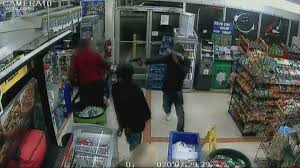
\includegraphics[width=0.8\linewidth]{fig/images}
	\end{multicols}
	\begin{multicols}{2}
		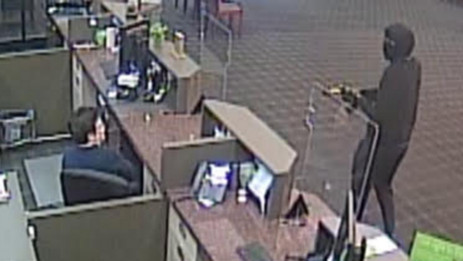
\includegraphics[width=0.8\linewidth]{fig/z5092842635515_66bf7170494f95e3b6d809a5e2e48128}
		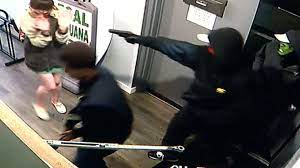
\includegraphics[width=0.8\linewidth]{fig/download}
	\end{multicols}
	\captionsetup{justification=centering}
	\caption{Hình ảnh thực tế trích xuất từ camera}
	\label{fig:example1}
\end{figure} 

Năm 2016, các nhà khoa học tại đại học California, Berkely \cite{ssd} đã giới thiệu một mô hình phát hiện vật thể hiện đại: Single Shot Multibox Detector (SSD). Mô hình đã đạt được kết quả rất tốt trên nhiều tập dữ liệu, cùng với tốc độ xử lý đạt mức thời gian thực nên được sử dụng rộng rãi trong các ứng dụng thực tế như phát hiện đối tượng trong ảnh y khoa, giám sát an ninh … Tuy nhiên, bên cạnh những điểm mạnh của mình, SSD vẫn gặp khó khăn trong việc phát hiện các vật thể nhỏ cũng như các bounding box hay bị mất đi trong quá trình xử lý video \cite{fpn, fpnssd}.Quay trở lại với bài toán phát hiện vật thể, việc phát hiện các vật thể các loại vũ khí là một thách thức vì chúng thường là các vật thể nhỏ (trong trường hợp súng lục, dao găm, …), đây cũng chính là điểm cần cải tiến của SSD, kèm với đó như đã đề cập, các bounding box không được giữ ổn định xuyên suốt quá trình nhận diện, nếu ta khắc phục được vấn đề này, ta có thể ứng dụng SSD vào trong bài toán nhận diện vũ khí và mong đợi đạt được kết quả khả quan. \\

Nhận thấy được tiềm năng cũng như với kết quả sơ khởi của ý tưởng cải tiến mô hình SSD, tôi quyết định chọn “Nghiên cứu và phát triển mô hình học sâu cho nhận diện và phân loại vũ khí sát thương” làm đề tài nghiên cứu của mình. Trong đề tài này, chúng tôi sẽ tập trung cải thiện các điểm yếu của SSD và ứng dụng mô hình đã cải tiến vào bài toán nhận diện vũ khí sát thương, thực hiện các phép đối chiếu và so sánh mô hình hiện tại (đã cải tiến) so với các mô hình truyền thống như hiện nay.


\section{\textbf{Cơ sở lý thuyết}}

\subsection{\textbf{Bài toán phát hiện vật thể}}
Trong lĩnh vực xử lí ảnh, bài toán phát hiện vật thể là đặt ra yêu cầu mô hình phải nhận diện được (khoanh vùng, tạo hộp giới hạn) một hoặc nhiều đối tượng từ các lớp đối tượng đã được huấn luyện từ trước trong một bức ảnh mà mô hình chưa từng đối mặt.Phát hiện vật thể đóng vai trò quan trọng trong nhiều ứng dụng thực tế, bao gồm nhận dạng khuôn mặt, nhận dạng biển số xe, phát hiện đối tượng trong video giám sát, gợi ý tag trong ứng dụng xã hội, và nhiều hơn nữa. Để giải quyết bài toán này, có nhiều phương pháp và thuật toán khác nhau đã được phát triển. Một trong những phương pháp phổ biến cho bài toán phát hiện vật thể là sử dụng các mô hình học máy dựa trên mạng học sâu tích chập. Ban đầu mô hình sẽ yêu cầu một tập dữ liệu huấn luyện đủ lớn đã bao gồm nhiều mẫu của các lớp đối tượng để có thể khái quát hóa đặc trưng của đối tượng đó, yêu cầu đặt ra là mô hình phải nhận diện được lớp đối tượng đã được huấn luyện từ trước từ những hình ảnh thực tế, không xuất hiện trong tập huấn luyện.

\begin{figure}[h]
	\center
	\begin{multicols}{2}
		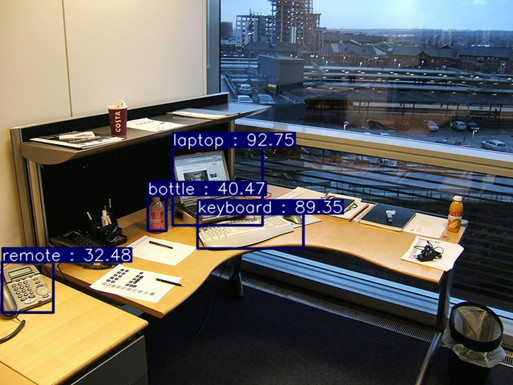
\includegraphics[width=0.8\linewidth]{fig/z5092846641905_ae48f72dcccc989ba3da7d5c9e133bdc}
		\includegraphics[width=0.89\linewidth]{fig/_150}
	\end{multicols}
	\captionsetup{justification=centering}
	\caption{Ví dụ về đầu ra của bài toán nhận diện vật thể}
	\label{fig:example2}
\end{figure} 

\subsection{\textbf{Ứng dụng và thách thức}}

Với sự phát triển của phần cứng máy tính, các phương pháp ứng dụng mạng học sâu đã trở nên khả thi trong thực tế, và nhận diện vật thể là một trong số đó. Có thể kể đến một vài ứng dụng nổi bật như : 

\begin{itemize}
	\item An ninh và giám sát: Phân loại đối tượng đóng vai trò quan trọng trong việc giám sát và bảo vệ an ninh tại các khu vực như sân bay, bến cảng, trạm xe buýt, tòa nhà công cộng và các khu vực quan trọng khác. Đóng vai trò nhận dạng các đối tượng có hành vi đáng ngờ hoặc nhận diện vật liệu nổ, vũ khí và các vật phẩm nguy hiểm khác.
	
	\item Ô tô tự hành: Nhận diện vật thể đóng vai trò quan trọng trong phát triển xe tự động. Nó giúp xe tự động nhận biết và phản ứng với các vật thể xung quanh như xe hơi, người đi bộ, xe đạp và các đối tượng khác trên đường. Tuy vẫn còn hạn chế về tốc độ xử lý khi so với phương pháp dùng cảm biến nhưng đây là một hướng nghiên cứu tiềm năng.
	
	\item Công nghiệp: Trong lĩnh vực công nghiệp, phân loại vật phẩm được sử dụng để kiểm tra chất lượng sản phẩm, phát hiện lỗi và đảm bảo quy trình sản xuất. Giúp xác định các chi tiết thiếu sót hoặc các thành phần không đúng quy cách trong quá trình sản xuất.
	
	\item Y tế: Phân loại vật thể có thể áp dụng trong lĩnh vực y tế để phát hiện các đối tượng y tế như khối u, bệnh lý và cấu trúc bất thường trong hình ảnh từ máy quét MRI, hỗ trợ chẩn đoán bệnh và đưa ra quyết định về điều trị.
	
	\item Thương mại điện tử: Trong lĩnh vực thương mại điện tử, phân loại vật phẩm giúp tìm kiếm và nhận dạng các sản phẩm trong hình ảnh, giúp người dùng dễ dàng tìm kiếm và mua sản phẩm. Ví dụ, người dùng có thể chụp hình ảnh sản phẩm và ứng dụng sẽ phân loại và tìm kiếm các sản phẩm tương tự trên các trang web mua sắm trực tuyến.
\end{itemize}

Tuy nhiên bên cạnh những ứng dụng rất tiềm năng thì việc ứng dụng phát hiện đối tượng vào thực tế cũng đối mặt với các thách thức, một số có thể kể đến như :

\begin{itemize}
	\item Đa dạng về hình dạng và kích thước: Vật thể có thể có nhiều hình dạng và kích thước khác nhau. Điều này đòi hỏi mô hình phát hiện vật thể phải có khả năng xử lý và nhận diện các đặc trưng đa dạng, từ các vật thể nhỏ như các vật dụng cầm tay cho đến các vật thể lớn có thể dễ nhận diện bằng mắt thường. Đồng thời, mô hình cũng cần đảm bảo khả năng phát hiện các vật thể có hình dạng biến đổi hoặc bị che khuất.

	\item Thay đổi ánh sáng và môi trường: Sự thay đổi về ánh sáng và môi trường có thể ảnh hưởng đến khả năng phát hiện vật thể. Ví dụ, ánh sáng yếu, bóng râm hoặc sự phản chiếu từ các bề mặt khác nhau có thể làm mờ hoặc che khuất vật thể. Yêu cầu mô hình phải có khả năng học và ứng dụng các đặc trưng chống nhiễu và chống lại sự ảnh hưởng thừ thay đổi ánh sáng.

	\item Số lượng lớn và đa dạng các lớp vật thể: Có hàng ngàn lớp vật thể khác nhau cần được phát hiện, từ động vật, đối tượng hàng hóa cho đến các nguyên tử. Điều này đặt ra một thách thức lớn trong việc huấn luyện mô hình phát hiện vật thể để có khả năng phân loại và nhận diện đa dạng các lớp vật thể một cách chính xác và hiệu quả.

	\item Che khuất và mất mát thông tin: Trong một số trường hợp, vật thể có thể bị che khuất hoặc mất mát thông tin trong hình ảnh. Các vật thể có thể bị che phủ bởi các vật thể khác, bóng đổ hoặc các vật thể chỉ hiển thị một phần. Điều này làm cho việc phát hiện vật thể trở nên khó khăn và đòi hỏi mô hình phải có khả năng nhận biết các đặc trưng phụ thuộc vào ngữ cảnh và xử lý các trường hợp che khuất và mất mát thông tin.
\end{itemize}

\subsection{\textbf{Các hướng tiếp cận hiện có}}
Cho đến nay các phương pháp tiếp cận cho bài toán nhận diện vật thể được chia làm hai hướng chính : two-stage detector và one-stage detector. Mỗi hướng nghiên cứu cố gắng tối ưu cho mục tiêu đặt ra của riêng chúng : tốc độ hoặc tính chính xác.

\begin{figure}[h]
	\centering
	\begin{subfigure}{0.45\textwidth}
		\centering
		\includegraphics[width=\linewidth]{fig/z5092886548627_508a1952da20813b18160ccc2a3c6d46}
		\caption{One-stage Detector}
		\label{fig:onestage}
	\end{subfigure}
	\begin{subfigure}{0.45\textwidth}
		\centering
		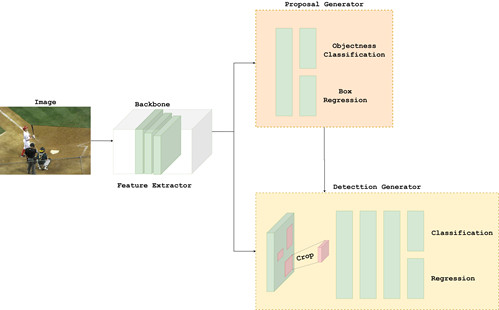
\includegraphics[width=\linewidth]{fig/z5092886306575_cdd8f127d1e80cf481c20b98939f77a9}
		\caption{Two-stage Detector}
		\label{fig:twostage}
	\end{subfigure}
	\captionsetup{justification=centering}
	\caption{Minh họa hai One-stage Detector và Two-stage Detector}
	\label{fig:combined}
\end{figure}

\textbf{Two-stage detector} :  Các mô hình theo phương pháp này được chia làm hai giai đoạn : giai đoạn đề xuất (proposal-stage) và giai đoạn phát hiện đối tượng (detection-stage). Ở giai đoạn đề xuất, mô hình chia ảnh thành các vùng đề xuất (region proposals) – nơi mà mô hình nghĩ rằng ở đó đang xuất hiện một vật thể nào đó. Sau đó các vùng đề xuất được đưa vào giai đoạn phát hiện đối tượng (Hình \ref{fig:twostage}), ở đây các lớp tích chập được dùng để trích xuất đặc trưng và ở bước cuối cùng, một bộ phân loại được dùng để tạo ra một vector xác suất cho mỗi một vùng đề xuất, đại diện cho xác suất xuất hiện của một vật thể trong vùng đề xuất đó. Các mô hình nổi bật trong hướng tiếp cận này có thể kể đến như R-CNN \cite{RCNN}, Fast R-CNN \cite{FRCNN}. Ưu điểm của phương pháp này là độ chính xác rất cao, đứng đầu trên các benchmark, tuy nhiên nhược điểm là tốc độ chậm, không đáp ứng được yêu cầu xử lí thời gian thực, do đó rất khó để có thể ứng dụng vào thực tiễn. \\

\textbf{One-Stage detector} : Ngược lại với two-stage detector, các mô hình họ one-stage chỉ gồm một giai đoạn duy nhất (Hình \ref{fig:onestage}). Ban đầu mô hình sẽ định nghĩa các hộp neo (anchor boxes) được cố định theo tỉ lệ trên hình ảnh gốc, các hộp neo này thay thế cho các vùng đề xuất trong mô hình two-stage. Hình ảnh ban đầu đi qua một loạt lớp tích chập, trích xuất được một bản đồ đặc trưng MxNxC, với M, N là kích thước của feature map và C là độ dài vector đặc trưng. Mỗi vector đặc trưng sẽ được gán cho một hộp neo đã đề cập ở trên. Sau đó cũng giống như two-stage detector, các vector đặc trưng này cũng sẽ được đi qua một bộ phân loại. Nhờ bỏ đi giai đoạn đề xuất và thay thế nó bằng các hộp neo được định nghĩa từ trước, họ mô hình one-stage có tốc độ rất nhanh, đáp ứng được thời gian thực nên rất được ưa chuộng, nhưng bù lại độ chính xác thua thiệt hơn two-stage-detector, tuy nhiên chênh lệch là không quá đáng kể. Đi đầu mô hình one-stage có thể kể đến như họ mô hình YOLO\cite{yolov1, yolov2, yolov3}, RetinaNet\cite{focalloss} hay SSD\cite{ssd}. \\

Mục tiêu của nghiên cứu là phát hiện sớm, ngăn chặn kịp thời các hành vi nguy hiểm nhờ vào phát hiện sự có mặt của những loại vũ khí mang tính sát thương cao. Do đó họ mô hình one-stage được chúng tôi lựa chọn làm hướng chính cho nghiên cứu này.

\subsection{\textbf{Mô hình phát hiện vật thể Single-Shot-Multibox Detector}}

Năm 2016, mô hình phát hiện vật thể một giai đoạn Single-Shot-Multibox Detector (SSD) \cite{ssd} được giới thiệu tới cộng đồng. SSD cũng áp dụng cơ chế mới mẻ : multi scale learning (Hình \ref{fig:SSD300}). Thay vì chỉ dùng feature map đầu ra ở layer CNN cuối cùng, SSD tận dụng những feature map đến từ những lớp CNN ở giữa. Với các feature map ở cuối, những vật thể to có thể được nhận diện tốt hơn do đi qua nhiều lớp tích chập, tuy nhiên điều này có thể làm mờ đi những đặc trưng của những vật thể nhỏ do tác động của lớp pooling max, do đó các feature map trung gian tỏ ra làm việc tốt hơn ở đối tượng có tỉ lệ nhỏ hơn. Với cơ chế multi scale learning, SSD cân bằng được độ chính xác lẫn tốc độ, đây là một ưu điểm lớn. Tuy nhiên SSD ứng dụng cơ chế này một cách khá đơn giản, chưa tận dụng được nhiều điểm mạnh của nó.

\begin{figure}[h]
	\centering
	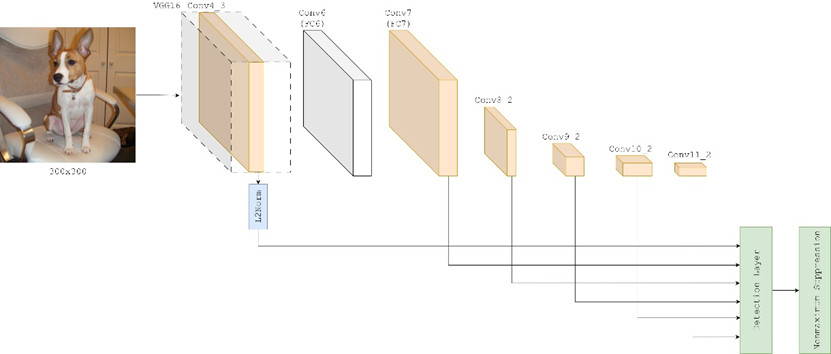
\includegraphics[width=0.9\linewidth]{fig/z5092846978629_cf95b8626921f76a1384d08ef3dcaa74}
	\caption{Kiến trúc của SSD áp dụng multiscale learning}
	\label{fig:SSD300}
\end{figure}

SSD có một kiến trúc khá đơn giản : một mạng trích xuất đặc trưng xương sống, các lớp tích chập bổ trợ và bộ phân loại đa tỉ lệ.

\begin{itemize}
	\item  \textbf{Mạng trích xuất đặc trưng xương sống} : một mạng được huấn luyện sẵn, có chức năng trích xuất được đặc trưng của ảnh. Trong bài báo gốc, nhóm tác giả dùng mạng VGG16 làm mạng xương sống.
	
	\item \textbf{Các lớp tích chập bổ trợ} : Nhằm phục vụ cho học tập đa tỉ lệ, nhóm tác giả đã thêm vào một vài lớp tích chập ở trên cùng của VGG16 nhằm trích xuất đặc đa tầng các bản đồ đặc trưng.
	
	\item \textbf{Bộ phân loại đa tỉ lệ} : Có nhiệm vụ dựa vào các bản đồ đặc trưng ở các lớp tích tập khác nhau đưa ra dự đoán về lớp và vị trí của đối tượng đó.
\end{itemize}

\subsection{\textbf{Feature Pyramid Network}}

Feature Pyramid Network (FPN) \cite{fpn} được giới thiệu lần đầu vào năm 2017 để giải quyết vấn đề của việc phát hiện đối tượng và phân vùng đa tỉ lệ. Trong các mạng nơ-ron tích chập truyền thống, các đặc trưng của hình ảnh được trích xuất thông qua các lớp tích chập và được mã hóa trong các tầng sau của mạng. Tuy nhiên, trong các tầng sâu, thông tin không gian chi tiết bị mất mát do quá trình gộp thông tin (downsampling). Điều này dẫn đến khả năng giảm hiệu suất của mạng trong việc phát hiện đối tượng ở các tỉ lệ khác nhau trong hình ảnh.

FPN được thiết kế để giải quyết vấn đề này bằng cách xây dựng một pyramidal hierarchy (Hình \ref{fig:FPN}) của các đặc trưng với các tỉ lệ khác nhau. Nó bao gồm hai thành phần chính: Bottom-up pathway và Top-down pathway.

\textbf{Bottom-up pathway} : bắt đầu từ hình ảnh gốc và sử dụng các lớp tích chập để trích xuất các đặc trưng từ các tầng sâu của mạng. Mỗi tầng sẽ tạo ra một bộ đặc trưng có độ phân giải khác nhau. Tuy nhiên, vì quá trình gộp thông tin, các bộ đặc trưng có độ phân giải cao sẽ mất thông tin không gian chi tiết.

\textbf{Top-down pathway} : bắt đầu từ các bộ đặc trưng có độ phân giải thấp và sử dụng các lớp upsampling để tăng kích thước của chúng. Sau đó, các bộ đặc trưng này được gộp với các bộ đặc trưng có độ phân giải cao từ Bottom-up pathway thông qua một phép cộng tương ứng pixel-wise. Quá trình này tạo ra một pyramidal hierarchy của các đặc trưng với thông tin không gian chi tiết từ các tầng thấp được truyền lên các tầng cao hơn.

\begin{figure}[h]
	\centering
	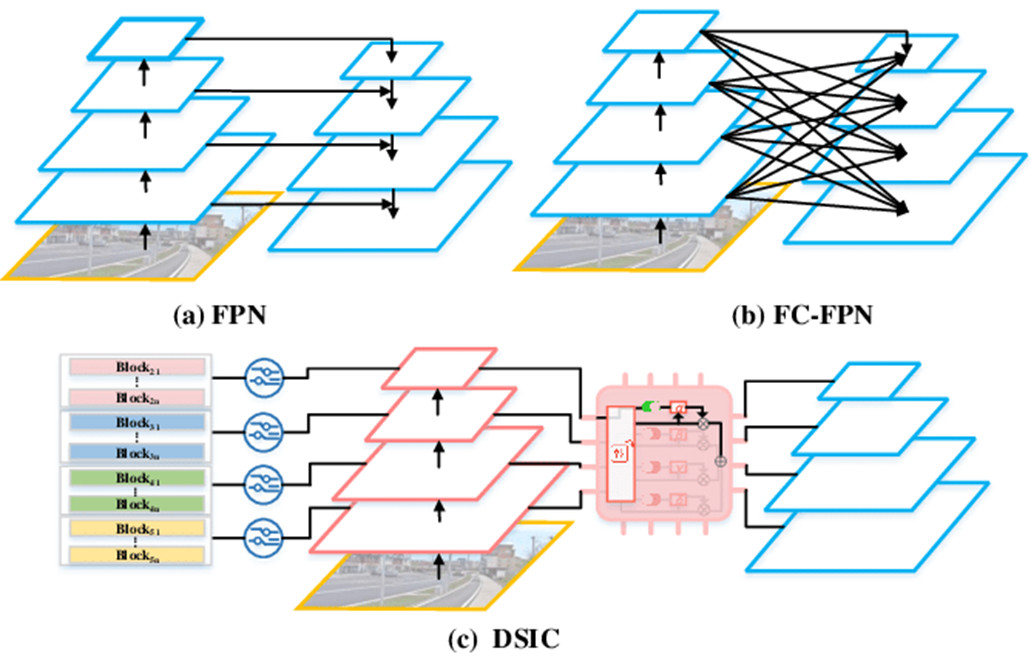
\includegraphics[width=0.7\linewidth]{fig/z5092847154512_f4e202b7896c8c37a42ed6fff62626c2}
	\caption{Một số ví dụ về cách thiết kế FPN}
	\label{fig:FPN}
\end{figure}


Kết quả là FPN cung cấp một pyramidal feature hierarchy với các bộ đặc trưng ở các tỉ lệ khác nhau, từ đó cho phép việc phát hiện đối tượng và phân vùng trên các vùng có độ phân giải khác nhau trong hình ảnh. Thêm vào đó, FPN còn giúp cải thiện hiệu suất của các mô hình phát hiện đối tượng, đảm bảo khả năng nhận diện chính xác ở các tỉ lệ khác nhau và đối phó tốt với các đối tượng có kích thước khác nhau trong hình ảnh. Tùy vào mục tiêu của người nghiên cứu mà cách kết hợp các feature map cũng có các cách thiết kế và độ phức tạp khác nhau, có thể thấy đây là phương pháp rất linh hoạt và khả năng tùy biến cao, dễ dàng ứng dụng vào những mô hình học sâu.

\subsection{\textbf{Mạng trích xuất đặc trưng VGG16}}

Khả năng nhận thức tự nhiên của con người cho phép chúng ta dễ dàng nhận biết các đối tượng thuộc cùng một loại dựa trên những đặc điểm chung của chúng. Ví dụ, ngay cả khi chưa từng thấy một giống chó cụ thể nào, chúng ta vẫn có thể nhận ra một con vật trong hình ảnh là một loài chó (mặc dù chúng ta có thể không biết chính xác là giống gì). Điều này cho thấy con người có khả năng nhận diện những đặc trưng của các đối tượng, mặc dù việc mô tả những đặc trưng này thường gặp khó khăn do tính trừu tượng của chúng. Từ quan sát này, ta có thể suy ra một hướng đi để giải quyết bài toán nhận diện đối tượng. Nếu chúng ta có một công cụ giúp lọc bớt thông tin dư thừa và chỉ tập trung vào những đặc trưng quan trọng, riêng biệt của các đối tượng, chúng ta có thể sử dụng những đặc trưng này để phân loại các đối tượng vào cùng một nhóm. Điều này cũng tương tự như cách con người nhận diện và phân loại các đối tượng dựa trên các đặc điểm chung của chúng.

Mạng tích chập (Convolutional Neural Network - CNN) là một công cụ quan trọng và mạnh mẽ được sử dụng rộng rãi trong việc trích xuất đặc trưng trong các bài toán nhận diện đối tượng. Hiện nay, hầu hết các mô hình học sâu đều sử dụng nhiều lớp tích chập kết hợp với nhau, cả về chiều rộng lẫn chiều sâu. Điều này cho phép mô hình học sâu nắm bắt được sự phức tạp và đa dạng của các đặc trưng trong dữ liệu. Lớp tích chập trong mạng CNN hoạt động bằng cách sử dụng phép tích chập, trong đó một bộ lọc (kernel) được áp dụng lên các vùng nhỏ của đầu vào để tạo ra các đặc trưng cục bộ. Bộ lọc này có thể tìm kiếm các thông tin cơ bản như góc, cạnh (Hình \ref{fig:edges}), hoặc các mẫu đặc trưng khác. Với mỗi bộ lọc khác nhau, lớp tích chập sẽ trích xuất được các đặc trưng khác nhau từ đầu vào. Một điểm đáng chú ý là các lớp tích chập trong mạng CNN không được định nghĩa từ trước. Thay vào đó, chúng được mô hình tinh chỉnh thông qua quá trình huấn luyện. Trong quá trình này, mô hình điều chỉnh trọng số của các bộ lọc để tối ưu hóa hiệu suất của mạng. Điều này cho phép mạng CNN tự động học cách trích xuất các đặc trưng có ý nghĩa từ dữ liệu huấn luyện. Với mỗi lớp tích chập tiếp theo, mạng CNN tiếp tục trích xuất các đặc trưng trừu tượng hơn và khó hiểu hơn đối với con người. Các bộ lọc ở các lớp sau này có khả năng tìm kiếm các mẫu phức tạp và các đặc trưng trừu tượng, giúp mô hình nhận diện và hiểu sâu hơn về các đối tượng trong dữ liệu. Kết quả sau khi áp dụng loạt các lớp tích chập này là một vector đặc trưng, được cho là chứa thông tin quan trọng về các đặc trưng của đối tượng ban đầu. Vector đặc trưng này thường có kích thước lớn và biểu diễn một cách trừu tượng các đặc trưng của đối tượng trong không gian đặc trưng. Sau đó, vector đặc trưng này được đưa vào một bộ phân loại (ví dụ: một mạng nơ-ron đầy đủ) để cung cấp thông tin chính xác về lớp của đối tượng đó.

\begin{figure}[h]
	\centering
	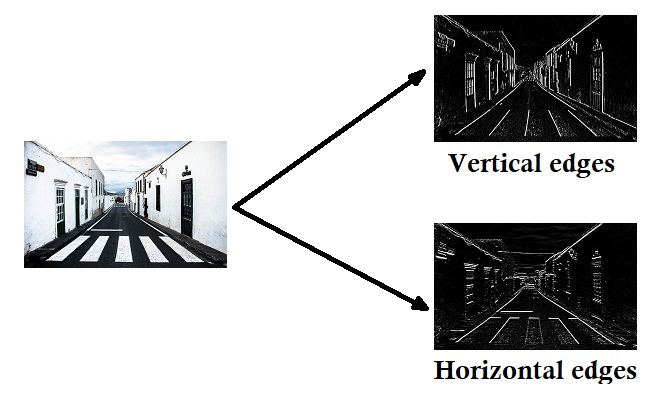
\includegraphics[width=0.7\linewidth]{fig/edges}
	\caption{Đầu ra của hai bộ lọc khác nhau}
	\label{fig:edges}
\end{figure}

VGG16 là một mạng nơ-ron tích chập sâu được sử dụng rộng rãi trong lĩnh vực thị giác máy tính, được đề xuất trong K. Simonyan và A. Zisserman từ University of Oxford trong bài báo \cite{vgg} như một công cụ mạnh mẽ để trích xuất đặc trưng từ hình ảnh. Với kiến trúc đơn giản và hiệu quả, VGG16 đã chứng minh khả năng của mình trong nhiều nhiệm vụ như nhận diện đối tượng, phân loại hình ảnh và phát hiện vật thể. Một trong những điểm nổi bật của VGG16 là kiến trúc sâu với tổng cộng 16 lớp, bao gồm 13 lớp tích chập và 3 lớp kết nối đầy đủ (Hình \ref{fig:network}). Các lớp tích chập của VGG16 được thiết kế với các bộ lọc nhỏ kích thước 3x3. Sử dụng các bộ lọc nhỏ này giúp mạng học được các đặc trưng cấp thấp và cấp cao từ hình ảnh, từ những đường cạnh và góc đến những đặc điểm phức tạp hơn như hình dạng và mẫu. Sau mỗi lớp tích chập, VGG16 sử dụng các lớp kích hoạt ReLU để đưa vào các giá trị dương và loại bỏ các giá trị âm, tăng tính phi tuyến và khả năng học của mạng. Các lớp tích chập được xếp chồng lên nhau liên tiếp để tạo ra một mạng sâu với khả năng học hiệu quả các đặc trưng từ hình ảnh. Sau các lớp tích chập, VGG16 sử dụng các lớp kết nối đầy đủ (fully connected layers) để kết hợp các đặc trưng đã được trích xuất thành một vector đặc trưng cuối cùng. Các lớp kết nối đầy đủ này hoạt động như một bộ phân loại, tìm hiểu mối quan hệ giữa các đặc trưng và phân loại chúng vào các lớp tương ứng. Một lợi ích quan trọng của VGG16 là khả năng tái sử dụng và chuyển giao đặc trưng. Với việc loại bỏ các lớp kết nối đầy đủ, VGG16 có thể được sử dụng như một mô hình trích xuất đặc trưng để trích xuất thông tin quan trọng từ hình ảnh mà không cần phải huấn luyện lại toàn bộ mạng. Điều này rất hữu ích trong các bài toán chuyển giao học tập (transfer learning), khi chúng ta có thể sử dụng VGG16 đã được huấn luyện trước trên một tác vụ lớn để trích xuất đặc trưng và sau đó chỉ cần huấn luyện một số lớp phân loại cuối cùng cho tác vụ cụ thể.

\begin{figure}[h]
	\centering
	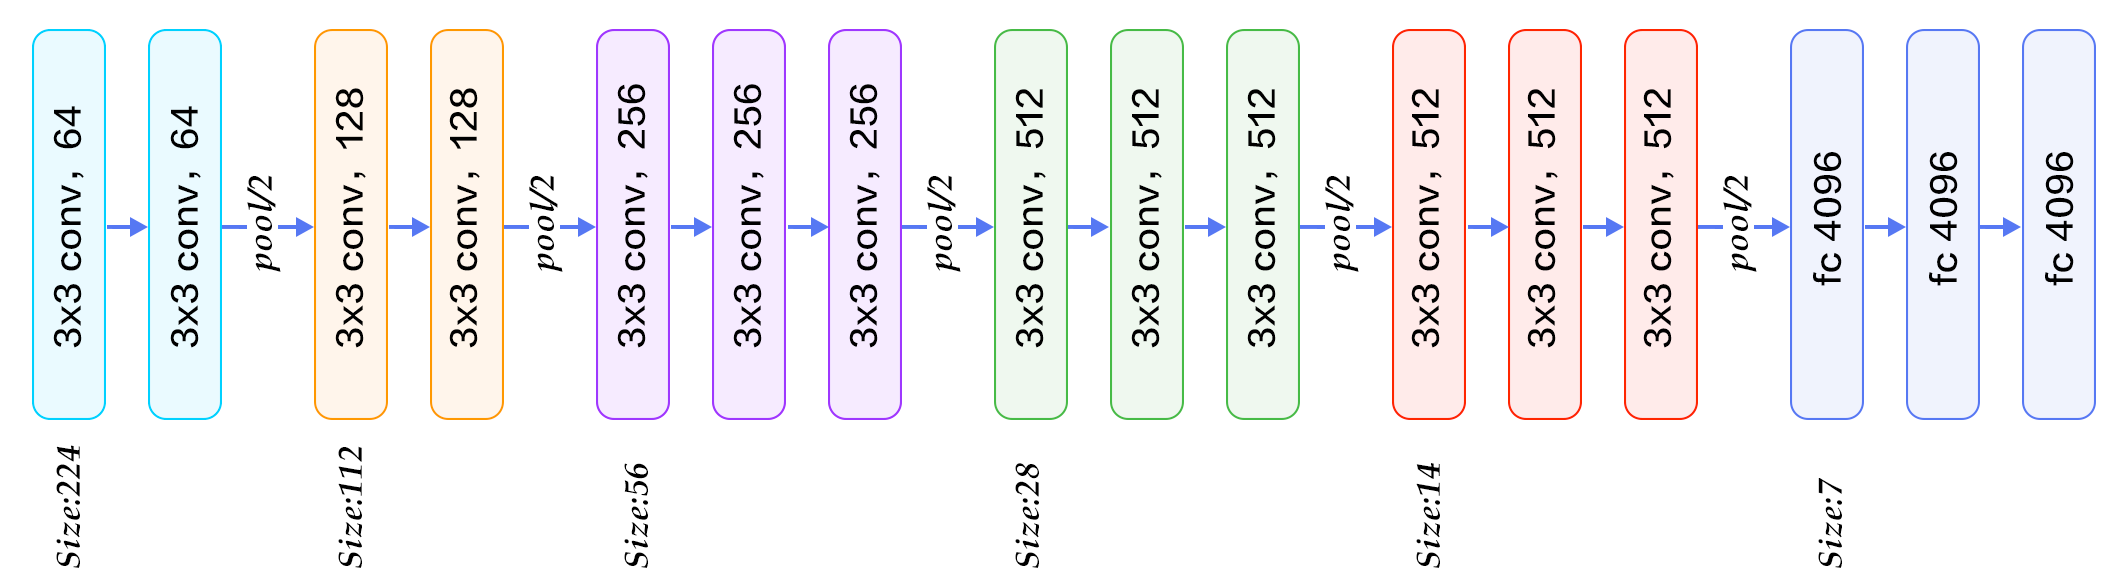
\includegraphics[width=0.9\linewidth]{fig/network}
	\caption{Kiến trúc của mạng VGG16}
	\label{fig:network}
\end{figure}

\section{\textbf{Đề xuất mô hình}}

\begin{figure}[h]
	\centering
	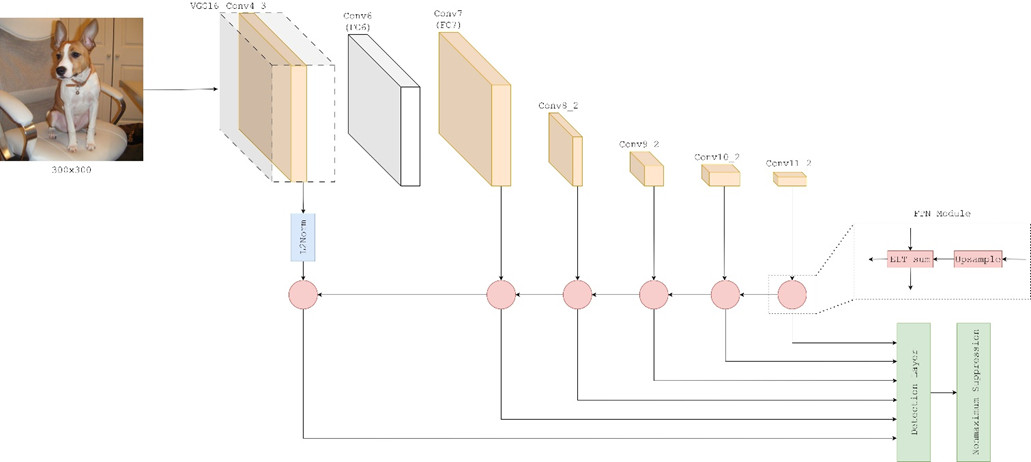
\includegraphics[width=0.9\linewidth]{fig/z5092847353686_14a2d2b2f8b64488c84035ba08549781}
	\caption{Kiến trúc của Lite FPN SSD}
	\label{fig:FPNSSD}
\end{figure}

\subsection{\textbf{Mạng xương sống và các lớp tích chập bổ trợ}}
Dựa vào mô hình SSD và mạng kim tự tháp, chúng tôi đề xuất một mô hình kết hợp và tận dụng điểm mạnh của cả hai kiến trúc kể trên, mô hình mới có tên là Lite FPN-SSD (Hình \ref{fig:FPNSSD}).
Cũng giống như SSD, Lite FPN-SSD cần một mạng xương sống nhằm trích xuất đặc trưng, ở đây chúng tôi dùng VGG16 cho mục đích này, một điểm khác biệt nhỏ là lớp fully connected 6 và 7 đã được chúng tôi lấy mẫu lại thành conv6 và conv7, vì vậy có tổng cộng 7 lớp tích chập trong mạng xương sống. Đầu tiên, hình ảnh được đi qua VGG16, đầu ra của nó là feature map Conv7,  tuy nhiên chúng tôi cũng giữ lại đầu ra của conv4 là Conv4 để xử lí ở các bước tiếp theo. Sau đó, Conv7 tiếp tục được đi qua các lớp tích chập bổ trợ là conv8, conv9, conv10 và conv11, lần lượt các đầu ra Conv8, Conv9, Conv10 và Conv11 cũng được giữ lại. Các phép tích chập ở trên đóng vai trò như bottom-up path trong FPN, sau cùng, chúng tôi có tổng cộng 6 feature map đó là Conv4, Conv7,  Conv8, Conv9, Conv10 và Conv11. 

\begin{table}[!htbp]
	\centering
	\caption{Thiết lập của các lớp tích chập từ mạng xương sống tới các lớp tích chập bổ trợ}
	\begin{tabular}{c|c|c|c|c|c|c}
		\toprule
		Name & in channels & out channels & kernel size & padding & stride & dilation \\
		\midrule
		conv1\_1 &   3  & 64   & 3 & 1 & 1 & 1 \\
		conv1\_2 &  64  & 64   & 3 & 1 & 1 & 1 \\
		conv2\_1 &  64  & 128  & 3 & 1 & 1 & 1 \\
		conv2\_2 & 128  & 128  & 3 & 1 & 1 & 1 \\
		conv3\_1 & 128  & 256  & 3 & 1 & 1 & 1 \\
		conv3\_2 & 256  & 256  & 3 & 1 & 1 & 1 \\
		conv3\_3 & 256  & 256  & 3 & 1 & 1 & 1 \\
		conv4\_1 & 256  & 512  & 3 & 1 & 1 & 1 \\
		conv4\_2 & 512  & 512  & 3 & 1 & 1 & 1 \\
		conv4\_3 & 512  & 512  & 3 & 1 & 1 & 1 \\
		conv5\_1 & 512  & 512  & 3 & 1 & 1 & 1 \\
		conv5\_2 & 512  & 512  & 3 & 1 & 1 & 1 \\
		conv5\_3 & 512  & 512  & 3 & 1 & 1 & 1 \\
		conv6    & 512  & 1024 & 3 & 6 & 1 & 6 \\
		conv7    & 1024 & 1024 & 1 & 1 & 1 & 1 \\
		conv8\_1 & 1024 & 256  & 1 & 0 & 1 & 1 \\
		conv8\_2 & 256  & 512  & 3 & 1 & 2 & 1 \\
		conv9\_1 & 512  & 128  & 1 & 0 & 1 & 1 \\
		conv9\_2 & 128  & 256  & 3 & 1 & 2 & 1 \\
		con10\_1 & 256  & 128  & 1 & 0 & 1 & 1 \\
		con10\_2 & 128  & 256  & 3 & 0 & 1 & 1 \\
		con11\_1 & 256  & 128  & 1 & 0 & 1 & 1 \\
		con11\_2 & 128  & 256  & 3 & 0 & 1 & 1 \\
		\bottomrule
	\end{tabular}%
	\label{tab:addlabel}%
\end{table}%

\subsection{\textbf{FPN Module}}

Để thực hiện top-down path, chúng tôi cần định nghĩa một phép tổng hợp thông tin của các feature map. Như đã thấy ở Hình \ref{fig:FPN} , có rất nhiều cách để thực hiện kết hợp feature map, tuy nhiên để không tác động đáng kể tới tốc độ của mô hình, chúng tôi lựa chọn cách thiết kế không quá phức tạp. Feature map từ tầng sâu sẽ được kết hợp với feature map từ tầng nông qua một module có tên là FPN module, đây là một module tùy biến, tức là tùy vào nhu cầu sử dụng mà có thể thay thế để tăng cường độ chính xác của mô hình. Tuy nhiên việc thiết kế module này không mang tính chất tuyến tính theo số lượng tham số (cứ nhiều tham số hơn là tốt hơn), để chứng minh nhận định trên chúng tôi tiến hành thử nghiệm với ba khác nhau là Moudule a, Module b và Module c (Hình \ref{fig:onestageandtwostage}), mức độ phức tạp tăng dần tương ứng, ở cả ba module phép eltsum được chọn đơn giản là cộng hai feature map lại với nhau :

\begin{itemize}
	\item \textbf{Moudle a} : Feature map ở lớp sâu được upsample với chế độ bilinear, đi qua lớp tích chập và sau đó là đi vào phép eltsum với đặc trưng nông (được giữ nguyên), sau cùng là đi qua lớp batch norm. 
	\item \textbf{Moudle b} : Đặc trưng ở sâu sẽ được upsample với chế độ bilinear, Đặc trưng nông sẽ được đi qua một lớp tích chập và batch norm, sau đó cả hai sẽ được kết hợp nhờ vào phép eltsum, sau cùng là một lớp tích chập và batch norm nữa.
	\item \textbf{Moudle c} : Đặc trưng ở sâu sẽ được upsample, đi qua một lớp tích chập, đặc trực ở nông được đi qua lớp tích chập, sau đó cả hai sẽ được kết hợp bằng phép eltsum.
\end{itemize}

\begin{figure} [h]
	\centering
	\begin{subfigure}{0.45\textwidth}
		\centering
		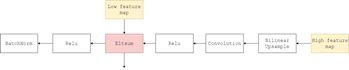
\includegraphics[width=0.7\linewidth]{fig/z5092847759693_0b41e43af0b0e40899f7c6db8b5e54b7}
		\caption{Moudle a : 27.6 triệu tham số}
		\label{fig:modulea}
	\end{subfigure}
	\begin{subfigure}{0.45\textwidth}
		\centering
		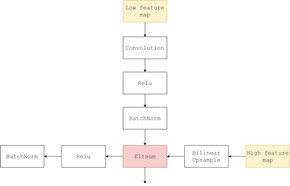
\includegraphics[width=0.7\linewidth]{fig/z5092847943183_94e9a29d3eb127c6d251749201fb7c7b}
		\caption{Module b : 28.3 triệu tham số}
		\label{fig:moduleb}
	\end{subfigure}
	\begin{subfigure}{0.45\textwidth}
		\centering
		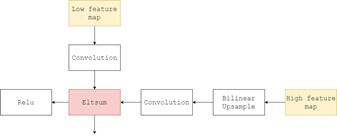
\includegraphics[width=0.7\linewidth]{fig/z5092848171130_735bb59cbabaaa9eb7e44a48ee39f110}
		\caption{Module c : 29.7 triệu tham số}
		\label{fig:modulec}
	\end{subfigure}
	\caption{One-stage Detector và Two-stage Detector}
	\label{fig:onestageandtwostage}
\end{figure}

Sau bước này, có tổng cộng 6 feature map được giữ lại và dùng cho bước nhận diện vật thể.

\section{\textbf{Tập dữ liệu}}

\subsection{The PASCAL Visual Object Classes (VOC)}

Pattern Analysis, Statistical Modelling, and Computational Learning (PASCAL) - một dự án nghiên cứu trong lĩnh vực học máy - đã tổ chức một chuỗi các cuộc thi dành cho phát hiện đối tượng : The PASCAL Visual Object Classes Challenge kéo dài từ năm 2005 tới 2012 với mục tiêu chính của  là nghiên cứu và phát triển các phương pháp và công cụ để giải quyết các vấn đề liên quan đến phân tích và nhận dạng hình ảnh. Trong suốt quá trình hoạt động, PASCAL VOC đã cung cấp các phiên bản của bộ dữ liệu VOC qua các năm nhằm làm một thang đo chung phục vụ cuộc thi. VOC bao gồm hàng ngàn hình ảnh đã được chú thích thu thập từ nhiều nguồn khác nhau. Các hình ảnh này bao gồm nhiều danh mục vật thể phổ biến như người, ô tô, động vật và các đối tượng khác. Mỗi hình ảnh trong tập dữ liệu được gắn kết với các nhãn và hộp giới hạn (bounding box) xác định vị trí của các vật thể trong hình ảnh. Phạm vi của tập dữ liệu VOC rất đa dạng, từ các hình ảnh trong môi trường ngoài trời đến các hình ảnh chụp trong môi trường trong nhà. Vào năm đầu tiên tổ chức, VOC với chỉ 4 lớp đối tượng bicycles, cars, motorbikes, people kèm theo 1578 bức ảnh chứa 2209 đối tượng đã được chú thích, VOC bắt đầu mở rộng quy mô lên con số 20 lớp với 11.530 bức ảnh và 27.450 đối tượng được chú thích.

\begin{figure}[h]
	\center
	\begin{multicols}{4}
		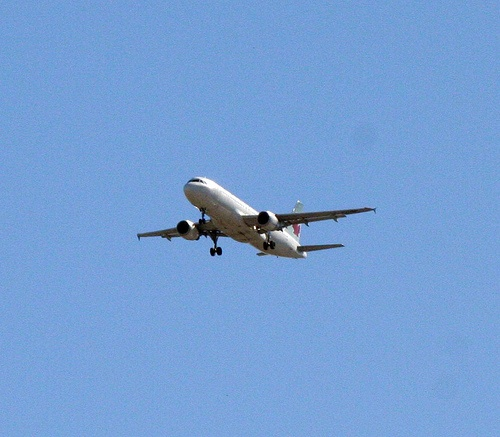
\includegraphics[width=0.7\linewidth]{fig/000665}
		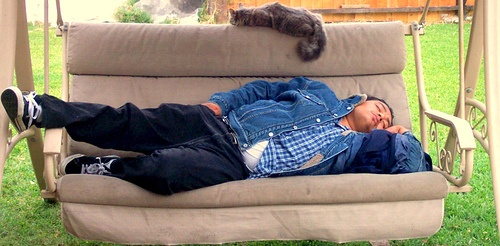
\includegraphics[width=1.\linewidth]{fig/000662}
		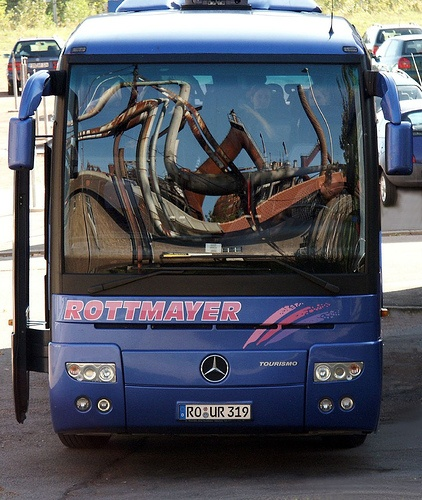
\includegraphics[width=0.7\linewidth]{fig/000663}
		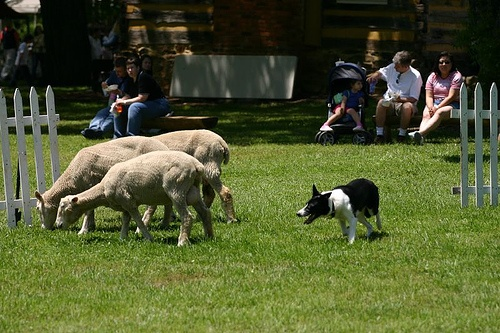
\includegraphics[width=1.\linewidth]{fig/000654}
	\end{multicols}
	\caption{Một số hình ảnh từ tập VOC}
	\label{exampleonVOC}
\end{figure}

\subsection{\textbf{Small Objects Handled Similarly to a weapon (SOHAS)}}

Được giới thiệu trong bài báo \cite{SOHAS}, đây là bộ dữ liệu được sử dụng cho mục đích phát hiện vũ khí và những vật thể cầm tay tương tự. Tập dữ liệu bao gồm sáu lớp : súng, điện thoại, dao, túi xách, tiền và thẻ. Nhóm tác giả sử dụng các camera giám sát khác nhau để thu thập hình ảnh, 10\% trong tổng số được tải về từ Internet. Tập dữ liệu này đóng vai trò quan trọng trong việc nâng cao hiệu suất của hệ thống giám sát video và đảm bảo an ninh công cộng.

\begin{figure}[h]
	\center
	\begin{multicols}{4}
		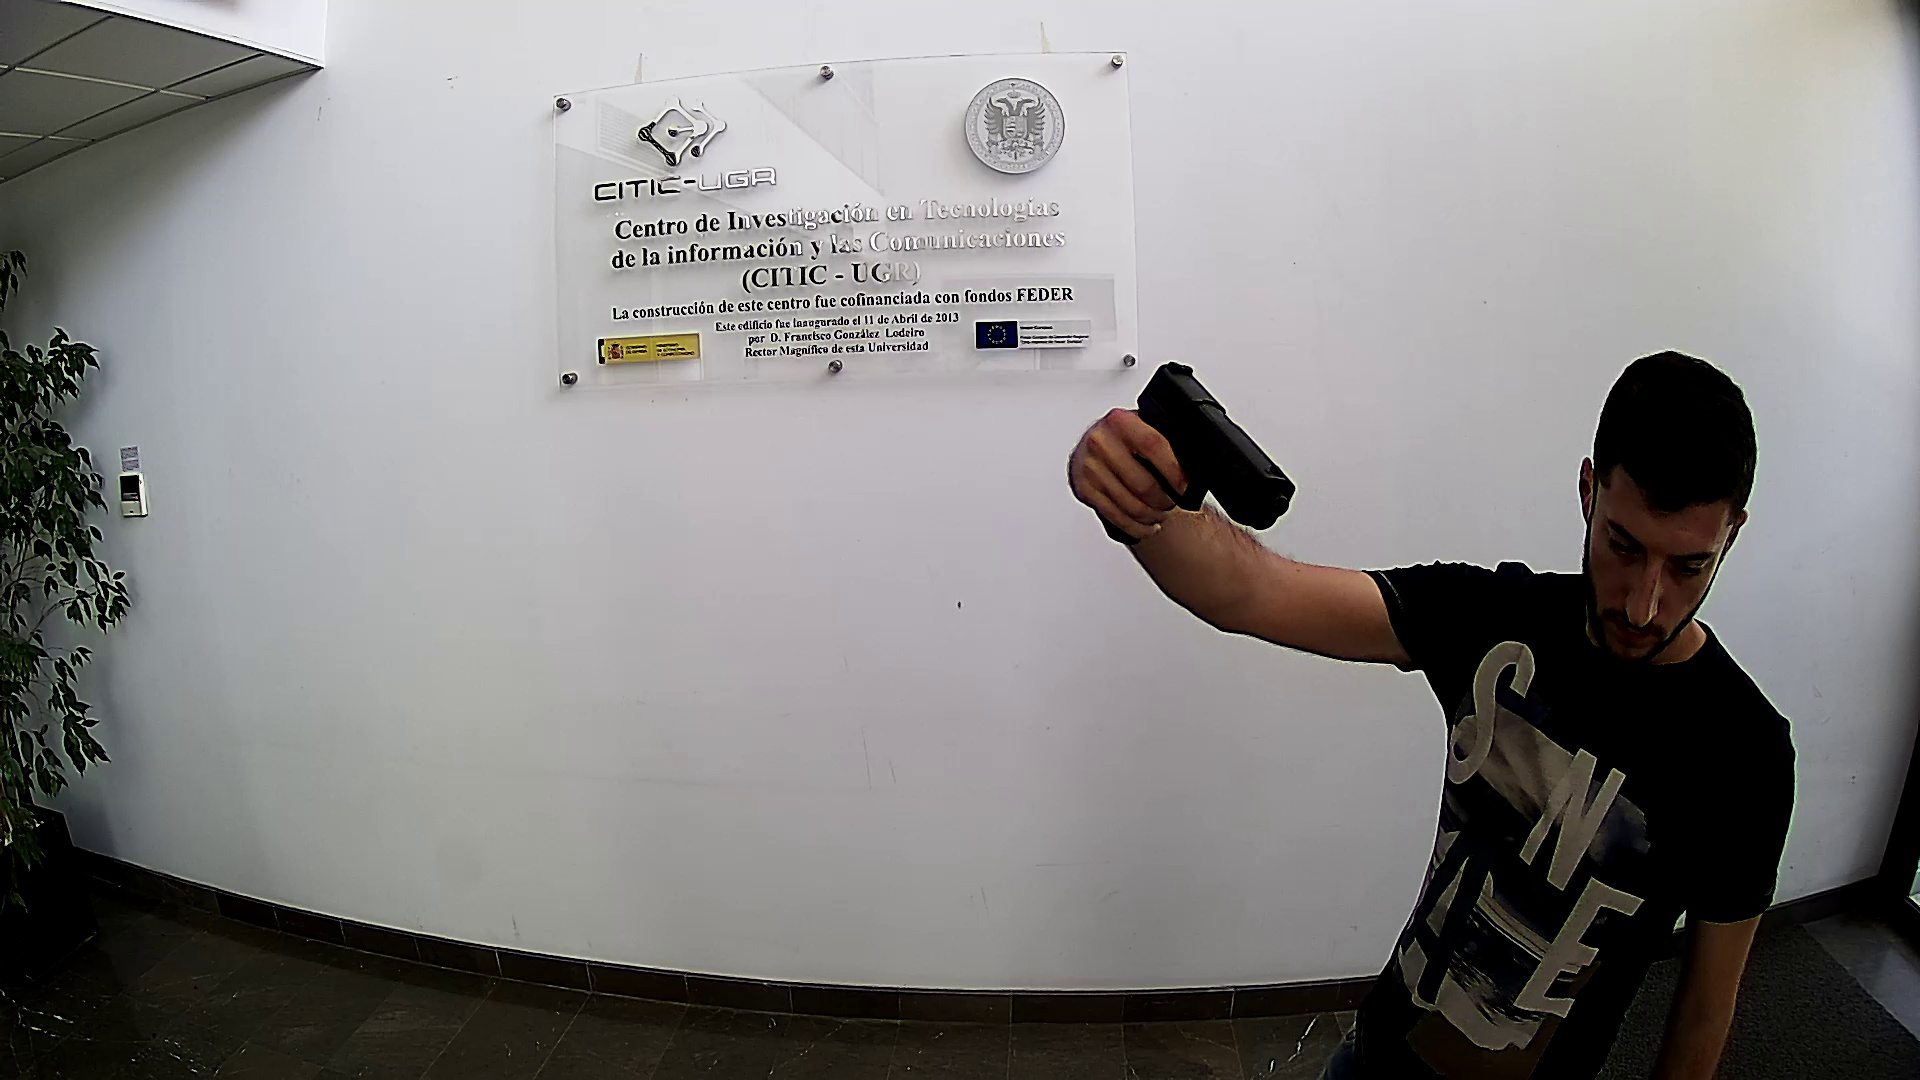
\includegraphics[width=0.9\linewidth]{fig/pistola_z3v5_09}
		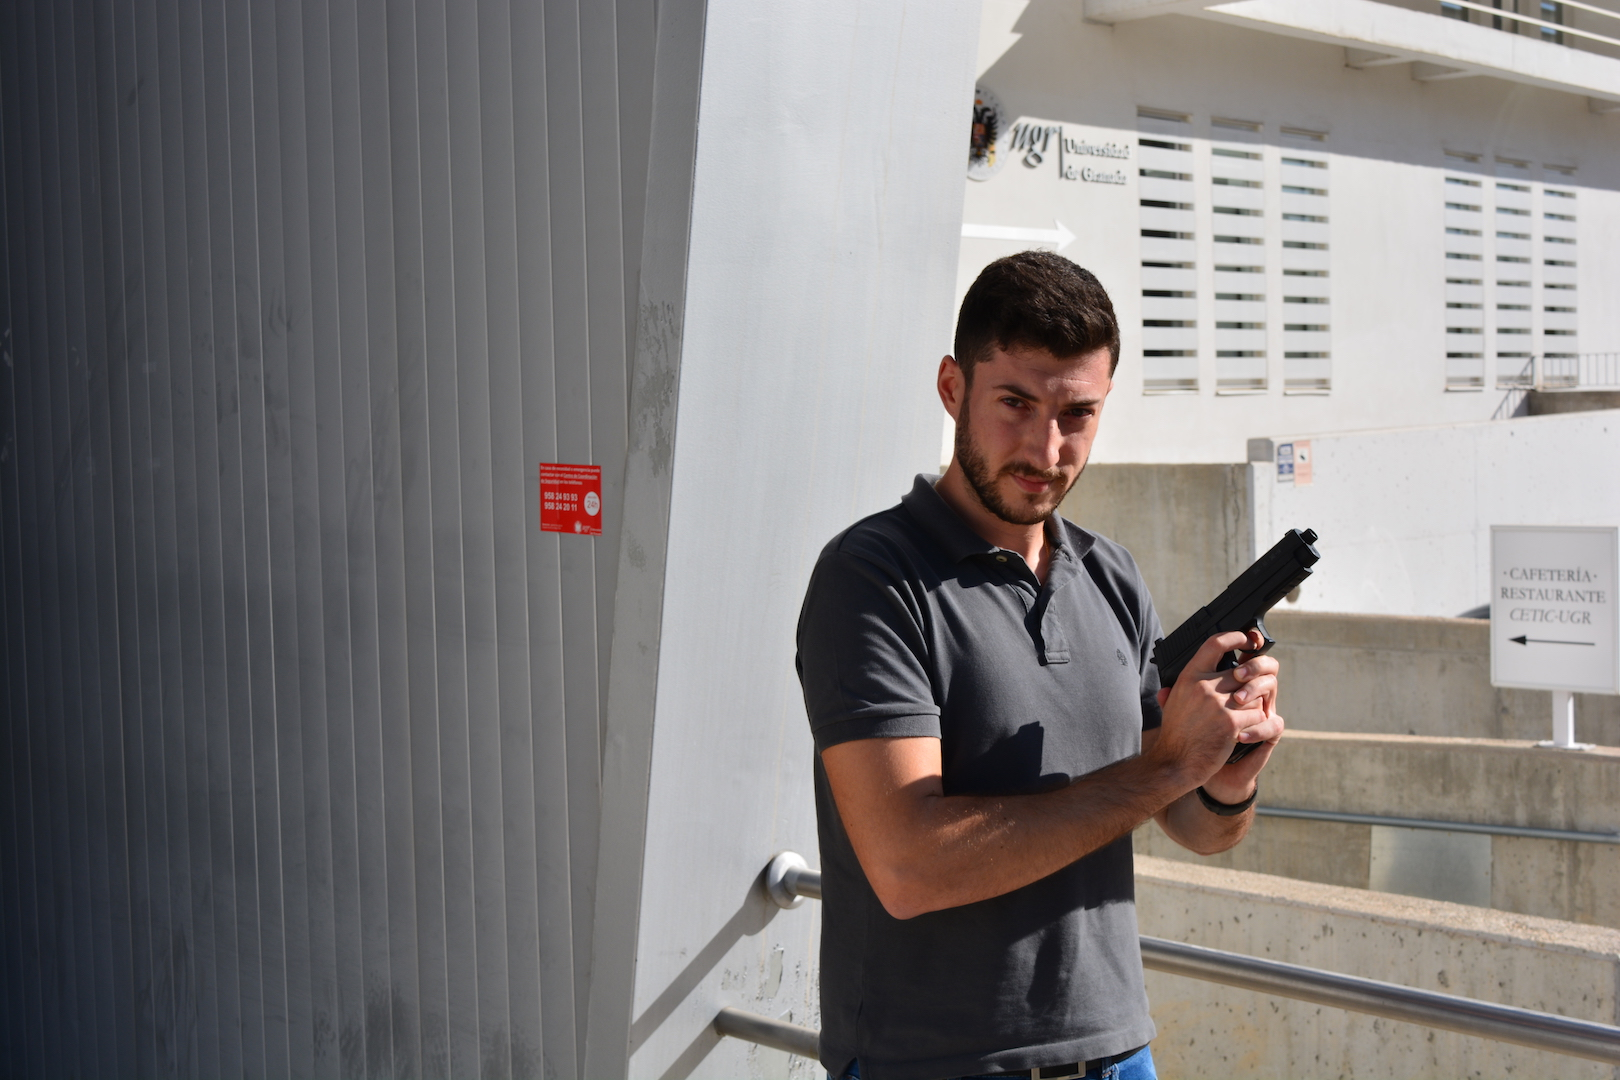
\includegraphics[width=0.9\linewidth]{fig/pistol_9047}
		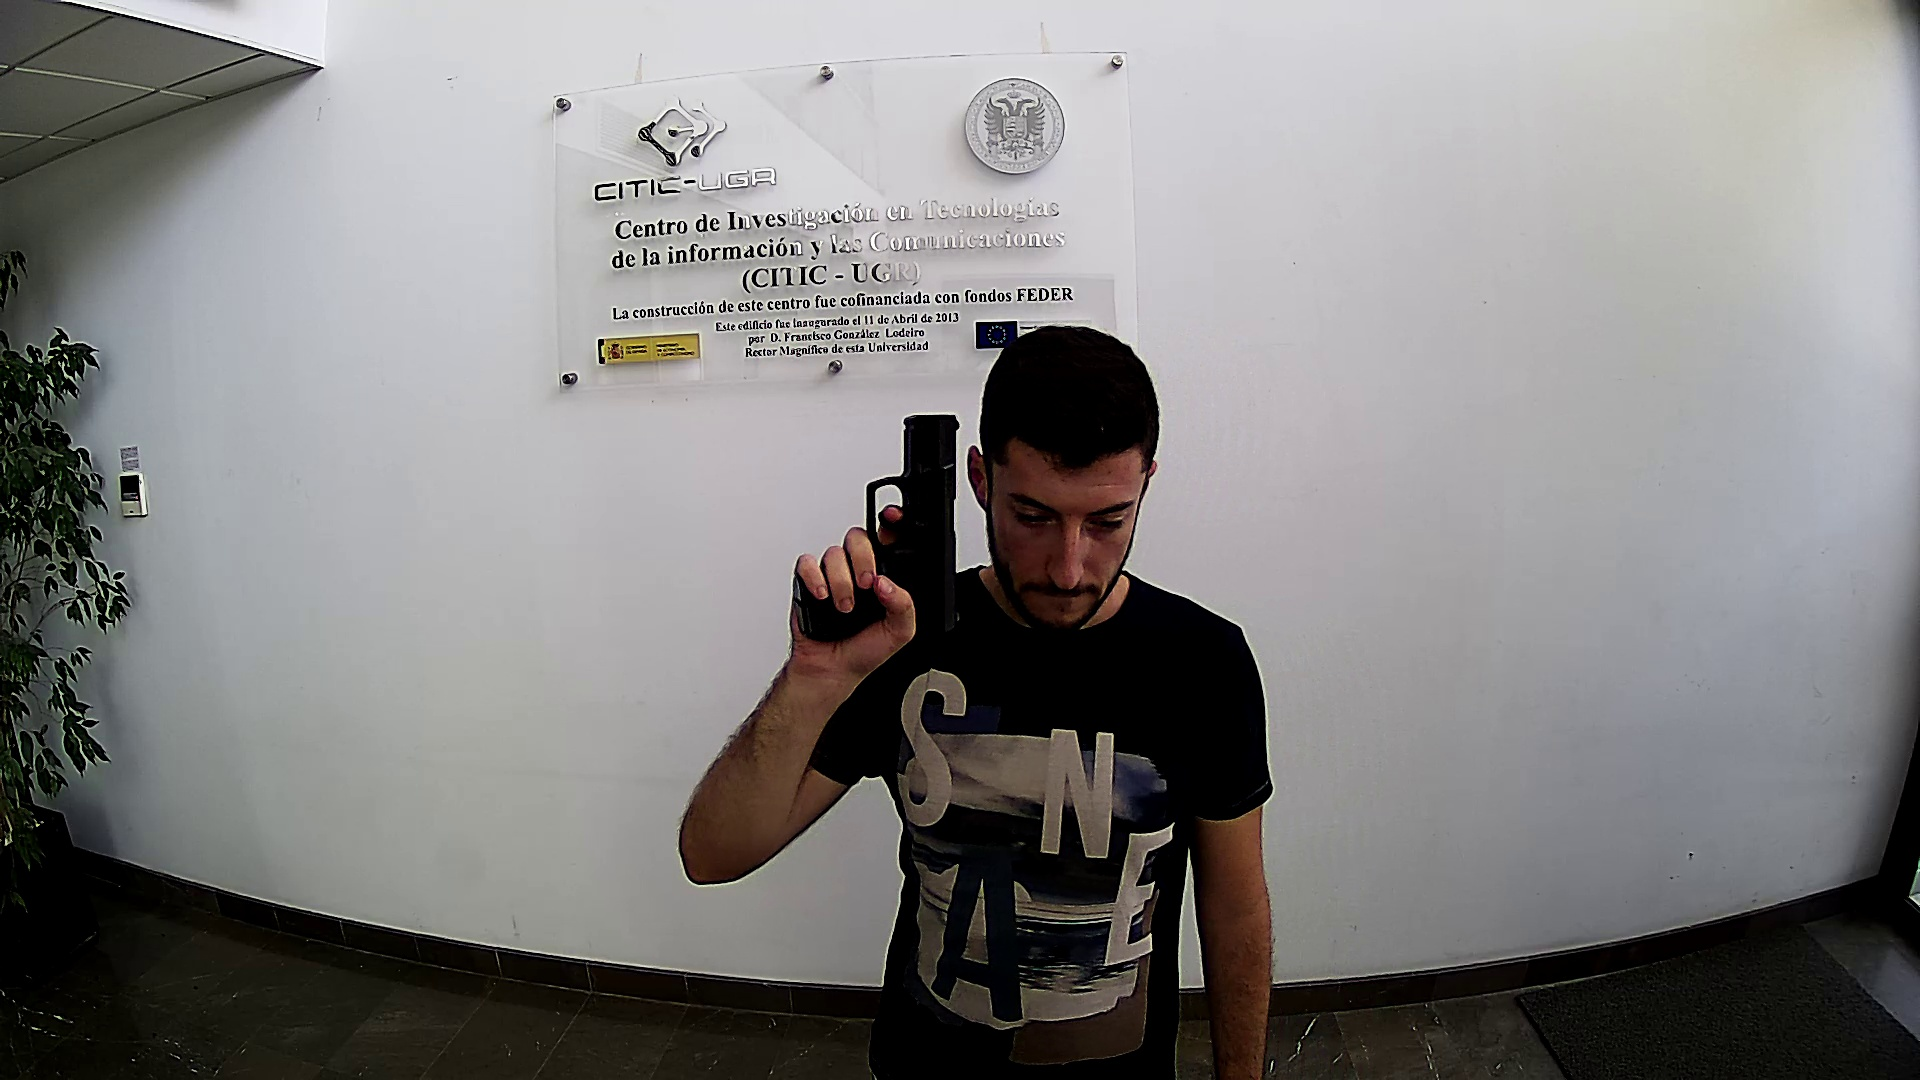
\includegraphics[width=0.9\linewidth]{fig/pistola_z3v3_09}
		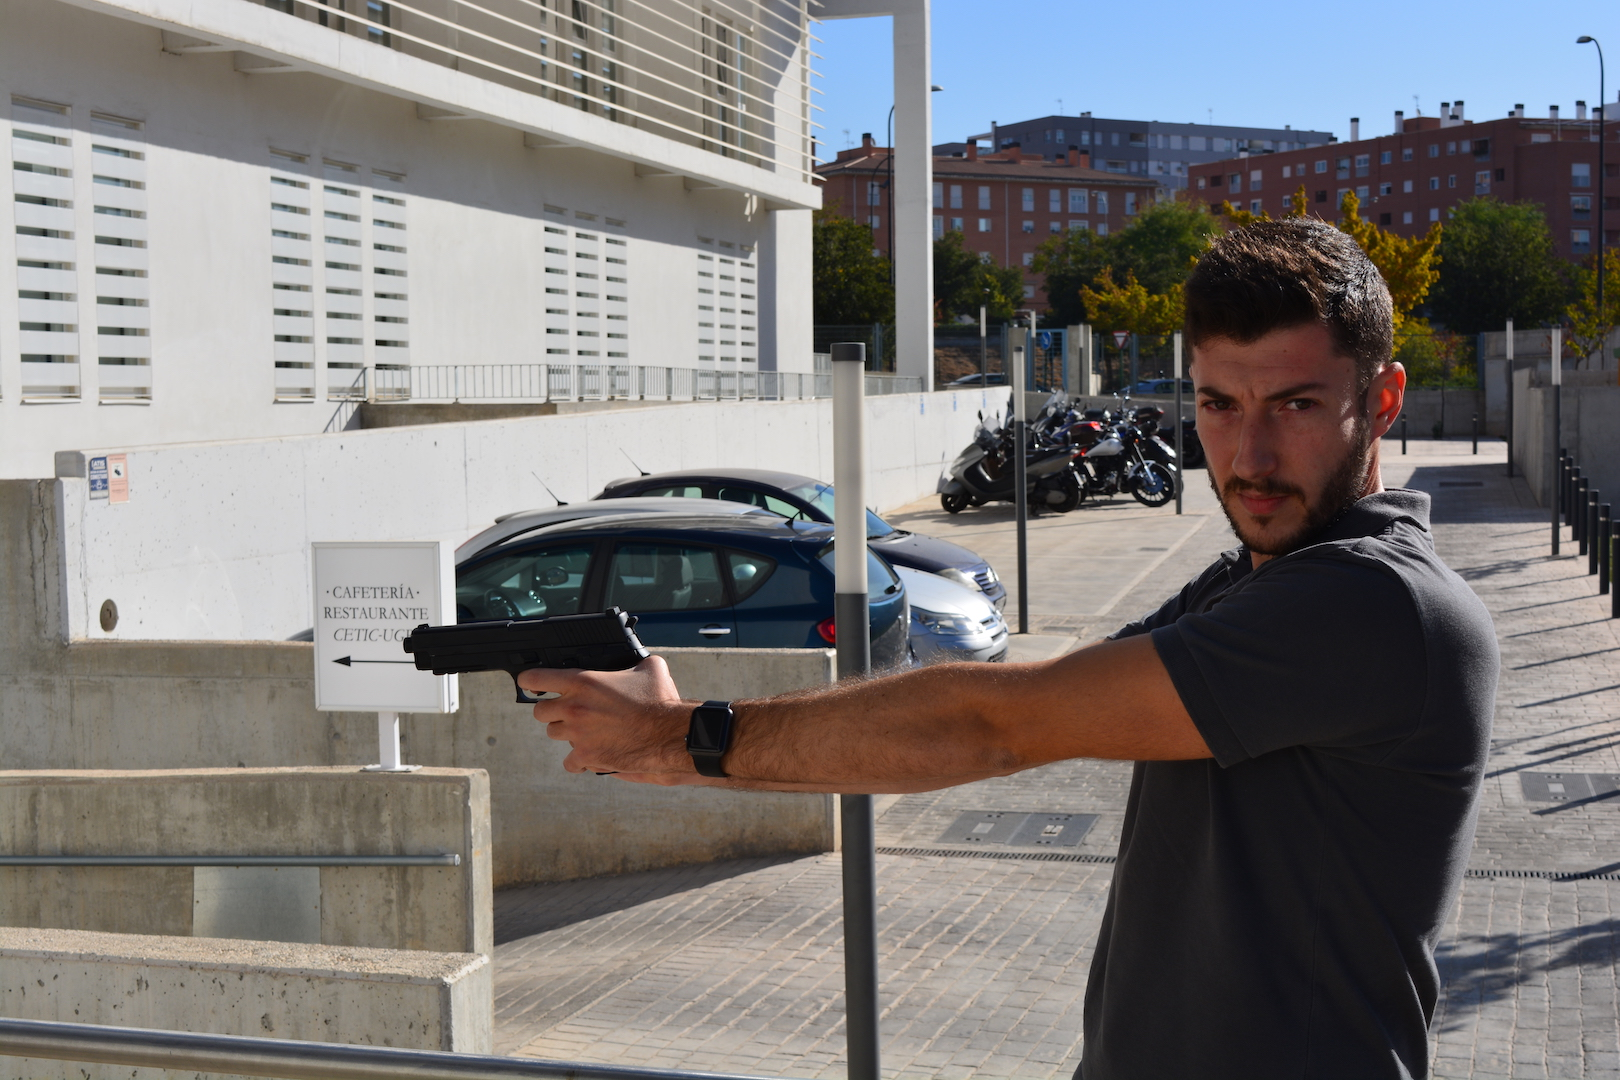
\includegraphics[width=0.9\linewidth]{fig/pistol_9048}
	\end{multicols}
	\caption{Một số hình ảnh từ tập SOHAS}
	\label{exampleonSOHAS}
\end{figure}


\section{\textbf{Thực nghiệm}}

\subsection{\textbf{Huấn luyện}}

\subsubsection{\textbf{Các hộp neo và tỉ lệ}}

Ban đầu, các hộp mặc định được thiết lập sẵn trên trên các ô của feature map, từ các hộp này, mô hình sẽ học cách dự đoán độ dời giữa các hộp mặc định và hộp thực tế, có thể thấy việc thiết lập các hộp mặc định là hoàn toàn thủ công, điều này là dựa vào mục đích sử dụng và đặc điểm của tập dữ liệu được dùng. Lần lượt các feature map conv4, conv7, conv8, conv9, conv10, conv11 có số lượng hộp trên từng ô là 4, 6, 6, 6, 4, 4. Tỉ lệ các hộp này được thiết lập theo công thức sau :

\begin{align*}
	w_k &= s_k \sqrt{a_k} \\
	h_k &= \frac{s_k}{\sqrt{a_k}}
\end{align*}

Với $w_k$ và $h_k$ là chiều rộng và chiều cao của anchor box, trong đó :
\begin{itemize}
	\item $s_k$ : được dùng để scale kích thước và là tham số tùy chọn cho từng tập dữ liệu.
	\item $a_k$ : tỉ lệ giữa chiều dài và chiều rộng của anchor box, $a_k \in \{1, 2, 3, 0.5, 0.333\}$
\end{itemize}



Ở bài báo gốc \cite{ssd}, tác giả thực tiện cắt các anchor box có phần thừa ra ngoài khung ảnh, tuy nhiên qua các thực nghiệm của mình, chúng tôi nhận thấy việc cắt đi các anchor box làm mất ổn định về vị trí của các hộp do thay đổi tâm và kích thước được định nghĩa sẵn ở một vài vị trí phần rìa, làm mAP bị giảm đi không quá 0.5 mAP, do đó chúng tôi giữ nguyên kích thước của các anchor box, điều này làm kết quả có xu hướng tốt hơn.

\subsubsection{\textbf{Hàm mục tiêu}}

Trước khi đi vào hàm mục tiêu, ta cần làm rõ một vài kí hiệu :

\begin{itemize}
	\item $x_{ij}^k$: một hàm chỉ số, trong đó $x_{ij}^p \in \lbrace 0, 1 \rbrace$. $x_{ij}^k = 1$ khi hộp neo $i$ được khớp với hộp thực tế (ground truth) $j$ cho lớp đối tượng $k$, $x_{ij}^k = 0$ trong trường hợp ngược lại.
	\item $\lbrace cx, cy, w, h \rbrace$: tương ứng đại diện cho tọa độ trung tâm theo trục ngang ($cx$) và trục dọc ($cy$), cũng như chiều rộng ($w$) và chiều cao ($h$) của một hộp neo. 
	\item $p$: độ dời được dự đoán bởi mô hình, biểu diễn dưới dạng $\lbrace \nabla{cx}, \nabla{cy}, \nabla{w}, \nabla{h} \rbrace$.
	\item $g$: giá trị thực tế (ground truth) $\lbrace cx, cy, w, h \rbrace$. 
	\item $d$: hộp neo, được biểu diễn dưới dạng $\lbrace cx, cy, w, h \rbrace$. 
	\item $c$: vector xác suất cho mỗi lớp, được ký hiệu là $\lbrace prob_1, prob_2, \ldots, prob_n \rbrace$. 
	\item $Pos$: tập hộp neo đã khớp được với một hộp thực tế. 
	\item $Neg$: tập hộp neo không được khớp. 
\end{itemize}

Chúng ta cần tối thiểu hàm mục tiêu sau : 

\begin{align}
	\mathcal{L}(p, d, g) &= \frac{1}{N}(\mathcal{L}_{conf}(c) + \alpha \mathcal{L}_{loc}(l, g)) 
\end{align} 

where $N$ represents the number of matched default boxes. If $N=0$, we assign a loss value of $0$. Here, $\alpha$ is a tunable parameter. The overall loss function $\mathcal{L}$ is the sum of two smaller component losses, $\mathcal{L}_{conf}$ and $\mathcal{L}_{loc}$.

Trong đó $N$ đại diện cho số lượng hộp neo được khớp. Nếu $N=0$, chúng ta gán giá trị hàm mất mát là $0$. Ở đây, $\alpha$ là một tham số có thể điều chỉnh. Hàm mất mát $\mathcal{L}$ là tổng của hai hàm mất mát nhỏ hơn, $\mathcal{L}{conf}$ và $\mathcal{L}{loc}$. \\

Hàm phạt cho việc xác định sai vị trí:

\begin{align}
	\mathcal{L}_{loc}(p, g) &= \sum_{i \in Pos}^{N} \sum_{m \in \lbrace cx, cy, w, h\rbrace} x_{ij}^{k} smooth_{L1}(p_i^m - \hat{g}_j^m)
\end{align} 

Cần lưu ý rằng ký hiệu $\hat{g}$ khác với $g$. Ở đây, $g$ đại diện cho tọa độ gốc, trong khi $\hat{g}$ biểu thị tọa độ chuẩn hóa sử dụng các công thức sau:

\begin{align}
	\hat{g}_j^{cx} &= \frac{(g_j^{cx} - d_i^{cx})}{d_i^w} \\ 
	\hat{g}_j^{cy} &= \frac{(g_j^{cx} - d_i^{cy})}{d_i^h} \\
	\hat{g}_j^w    &= \log(\frac{g_j^w}{d_i^w}) \\
	\hat{g}_j^h    &= \log(\frac{g_j^h}{d_i^h})
\end{align}

Hàm mất mát cho độ tự tin (xác suất):

\begin{align}
	\mathcal{L}_{conf}(c) = - \sum_{i \in Pos}^N x_{i, j}^k \log(\hat{c}_i^k) - \sum_{i \in Neg} log(\hat{c}_i^0), \\
	 ~ where ~ \hat{c}_i^k = \frac{\exp(c_i^k)}{\sum_{k} \exp(c_i^k)}
\end{align}


Bằng cách tối thiểu hóa các thành mất mát này, chúng ta có thể tối ưu hóa hiệu quả hàm mất mát tổng thể, từ đó giúp định vị đối tượng chính xác và ước lượng độ tin cậy. \\

\subsection{\textbf{Phương pháp đánh giá}}

Chúng tôi sử dụng thang đo mean average precision 0.5 (mAP:0.5) để đánh giá mô hình, trong phần này chúng tôi sẽ trình bày cách tính mAP thông qua các khái niệm liên quan.

\subsubsection{\textbf{Intersect over Union}}

\begin{figure}[h]
	\centering
	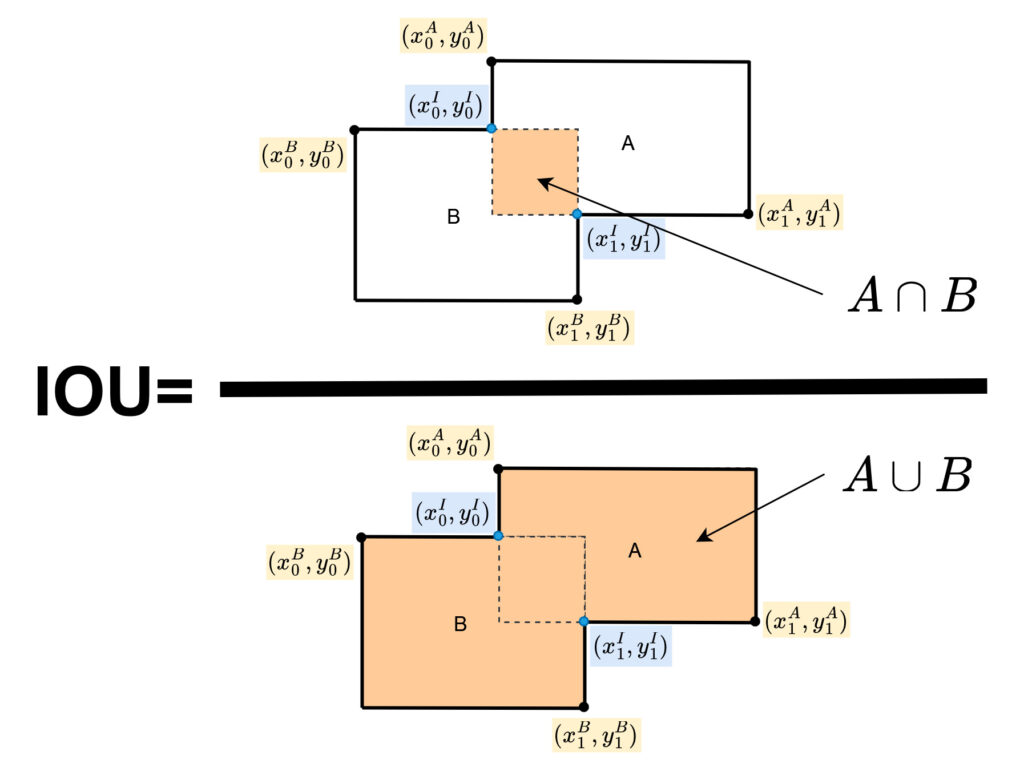
\includegraphics[width=0.5\linewidth]{fig/IOU3-1024x784}
	\caption{Minh họa cách tính IoU}
	\label{fig:iou3-1024x784}
\end{figure}

Còn được gọi là Jaccard index, là một phép đo được sử dụng để đánh giá mức độ trùng lắp giữa hai tập hợp hay hai vùng quan tâm. Trong ngữ cảnh của phát hiện vật thể, IoU được sử dụng để so sánh sự chồng lấp giữa một vùng quan tâm dự đoán (vùng quan tâm đã được phân loại hoặc định vị bằng mô hình) và một vùng quan tâm thực tế (vùng quan tâm được gán nhãn bởi con người). IoU đo lường tỷ lệ giữa diện tích vùng quan tâm được dự đoán và diện tích vùng quan tâm thực tế đã gán nhãn.

Công thức tính IoU cho hai tập hợp A và B được định nghĩa như sau: 
\begin{align*}
	IoU = \frac{\text{Diện tích giao nhau của A và B}}{\text{Diện tích hợp của A và B}}
\end{align*}


Trong đó, diện tích giao nhau là diện tích của phần chung giữa hai vùng quan tâm, và diện tích hợp là tổng diện tích của cả hai vùng quan tâm.

Giá trị IoU nằm trong khoảng từ 0 đến 1, với 0 nghĩa là không có sự trùng lắp giữa hai vùng quan tâm và 1 đại diện cho sự trùng lắp hoàn toàn. Điều này cho phép đánh giá chính xác mức độ trùng lắp giữa các vùng quan tâm và đo lường hiệu suất của các mô hình phân đoạn.

\subsubsection{\textbf{True Positive và False Positive}}

\begin{figure}[h]
	\centering
	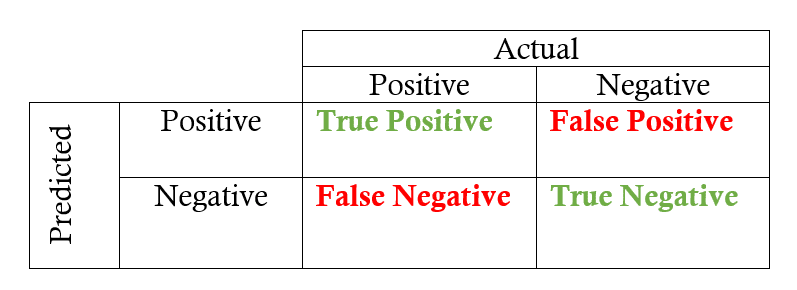
\includegraphics[width=0.7\linewidth]{fig/positive-negative-true-false-matrix}
	\caption{Minh họa trực quan về True Positive, True Negative, False Positive và False Negative}
	\label{fig:positive-negative-true-false-matrix}
\end{figure}

Các khái niệm True Positive, True Negative, False Positive và False Negative được là các thuật ngữ được sử dụng để mô tả kết quả của một hệ thống phân loại hoặc mô hình. Trong ngữ cảnh phát hiện vật thể, các thuật ngữ này có thể được giải thích như sau :
\begin{itemize}
	\item True Positive : Mô hình dự đoán có một vật thể nằm ở đó và thật sự là như vậy.
	\item  True Negative : Mô hình dự đoán rằng không có vật thể nào ở đó và thật sự là như vậy.
	\item False Positive : Mô hình dự đoán có một vật thể nằm ở đó nhưng thật sự không có.
	\item False Negative : Mô hình dự đoán rằng không có vật thể nằm ở đó nhưng thật sự là có.
\end{itemize}

\subsubsection{\text{Độ chính xác và độ phủ (Precision và Recall)}}

Precision và Recall là hai phép đo quan trọng được sử dụng để đánh giá hiệu suất của các hệ thống phân loại hoặc mô hình trong lĩnh vực xử lý ảnh, thị giác máy tính và các bài toán phân loại.

Precision (độ chính xác): Precision đo lường tỷ lệ giữa số lượng dự đoán đúng thuộc một lớp cụ thể và tổng số lượng dự đoán thuộc lớp đó. Nó đo lường khả năng của mô hình xác định chính xác các mẫu thuộc lớp quan tâm. Precision được tính bằng công thức:

\begin{align*}
	Precision = \frac{\text{True Positive}}{\text{True Positive + False Positive}}
\end{align*}

Recall (độ nhạy, độ phủ): Recall đo lường tỷ lệ giữa số lượng dự đoán đúng thuộc một lớp cụ thể và tổng số lượng mẫu thực tế thuộc lớp đó. Nó đo lường khả năng của mô hình phát hiện được tất cả các mẫu thuộc lớp quan tâm. Recall được tính bằng công thức:

\begin{align*}
	Recall = \frac{\text{True Positive}}{\text{True Positive + False Negative}}
\end{align*}

Trong đó, True Positive là số lượng dự đoán đúng thuộc lớp quan tâm và False Negative là số lượng mẫu thực tế thuộc lớp quan tâm bị dự đoán sai.

\begin{figure}[h]
	\centering
	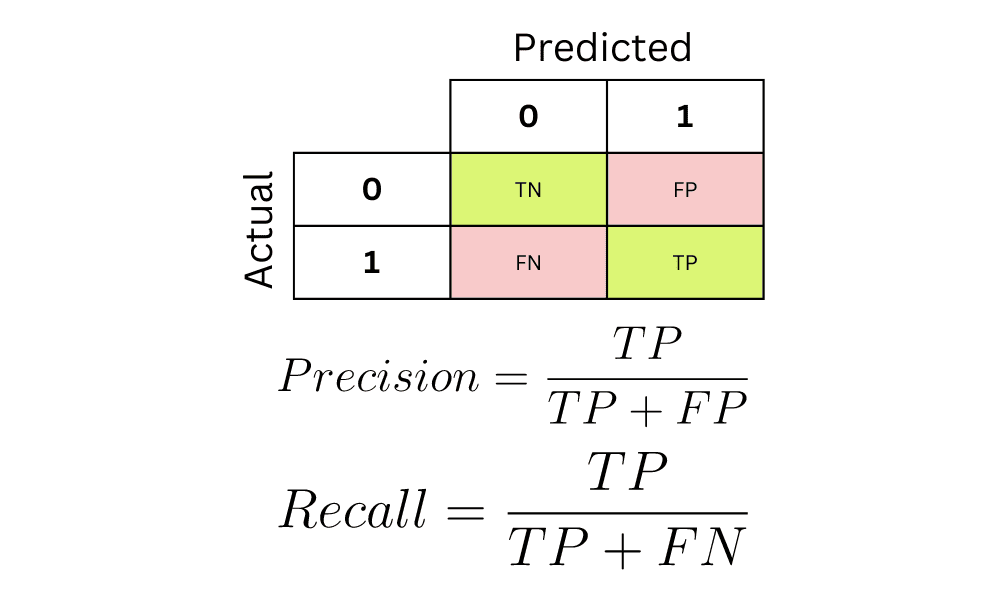
\includegraphics[width=0.7\linewidth]{fig/selvaraj_confusion_matrix_precision_recall_explained_12}
	\caption{Cách tính Precision và Recall}
	\label{fig:selvarajconfusionmatrixprecisionrecallexplained12}
\end{figure}

Precision và Recall thường có một mối quan hệ đối lập. Khi tăng giá trị ngưỡng IoU để quyết định xem một mẫu được coi là đượ khớp, mô hình có thể đạt được precision cao hơn nhưng recall thấp hơn. Ngược lại, khi giảm giá trị threshold, mô hình có thể đạt được recall cao hơn nhưng precision thấp hơn. Do đó, precision và recall thường được sử dụng cùng nhau để đánh giá hiệu suất tổng thể của một hệ thống phân loại hoặc mô hình.



\subsubsection{\textbf{Đường cong precision-recall }}

Precision-Recall curve (đường cong Precision-Recall) là một biểu đồ biểu thị mối quan hệ giữa recall và precision cho các mô hình phân loại hoặc hệ thống trong lĩnh vực xử lý ảnh, thị giác máy tính và các bài toán phân loại. Đồ thị PR có trục tung là Precision, trục hoành là Recall thường là một đường cong xuống.

\begin{figure}[h]
	\centering
	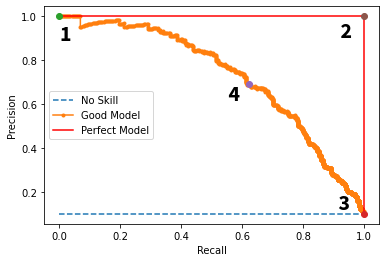
\includegraphics[width=0.5\linewidth]{fig/good.png-mh}
	\caption{Ví dụ về đồ thị precision-recall}
	\label{fig:good}
\end{figure}

Có thể đánh giá một mô hình phân loại dựa trên đồ thị PR : kẻ một đường thẳng từ điểm (0, 1) tới điểm (1, 0), nếu đường cong nằm càng trên đường này (tức hướng về điểm (1, 1)) thì mô hình càng tốt, ngược lại nếu đường cong nằm càng dưới đường này (tức hướng về điểm (0, 0)) thì mô hình càng không tốt. Có thể tính diện tích dưới đường cong PR để suy ra điều tương tự.

Để vẽ được đường cong này, trước hết chúng ta khớp các hộp dự đoán với các hộp thực tế, nếu khớp, ta xem đấy là một True Positive, nếu không, ta xem đấy là một mẫu False Positive. Sau đó sắp xếp các hộp dự đoán theo thứ tự giảm dần của độ tự tin. Gọi $N$ là số lượng hộp dự đoán, $M$ là số lượng hộp thực sự, ta cần tính hai vector vec-Precision và vec-Recall. Công thức tính được cho như sau : 

\begin{align*}
	\text{vec-Precision}[i] &= \frac{\sum_{j=1}^{i}{\text{TP}[j]}}{i} \\
	\text{vec-Recall}[i]    &= \frac{\sum_{j=1}^{i}{\text{TP}[j]}}{M} \\
\end{align*}

Trong đó TP$[i] = 1$ nếu hộp dự đoán $i$ là True Positve, và bằng $0$ trong trường hợp ngược lại.
Tới đây ta đã vẽ được đồ thị Precision-Recall với trục hoành là vec-Recall và trục tung là vec-Precision.

\subsubsection{Mean Average Precision (mAP)}

mAP là một phép đo quan trọng vì nó cho phép xem xét chất lượng phân loại trên tất cả các lớp và tính toán một chỉ số tổng quan cho hiệu suất trung bình trên tất cả các lớp. Nó cung cấp cái nhìn tổng quan và toàn diện về hiệu suất của mô hình trong các bài toán phân loại đa lớp hoặc phân đoạn vùng quan tâm. mAP thường được sử dụng trong các lĩnh vực như nhận dạng đối tượng, phát hiện vật thể và nhận dạng hành động trong thị giác máy tính. Ở đây chúng tôi sử dụng mAP:0.5, để tính được mAP:0.5, chúng ta thực hiện các bước sau :

\begin{itemize}
	\item Chọn ngưỡng IoU = 0.5.
	\item Với mỗi lớp trong $C$ lớp đang quan tâm : Vẽ đồ thị PR, tính diện tích dưới đường cong PR.
	\item mAP = trung bình tất cả các diện tích dưới đường cong PR của các lớp.
\end{itemize}

\subsubsection{\textbf{Tăng cường dữ liệu}}

Để cải thiện quá trình huấn luyện và nâng cao khả năng của mô hình trong việc phát hiện đối tượng, chúng ta sử dụng một số kỹ thuật tăng cường dữ liệu :

\begin{itemize}
	\item Điều chỉnh ngẫu nhiên: Hình ảnh được điều chỉnh ngẫu nhiên về độ sáng, độ tương phản, độ bão hòa màu và màu sắc. Mỗi sự điều chỉnh có 50\% khả năng được áp dụng, và thứ tự là ngẫu nhiên.
	
	\item Phóng to: Với xác suất 50\%, thực hiện phép phóng to hình ảnh từ 1 đến 4 lần. Các khoảng trống điền bằng giá trị trung bình của dữ liệu ImageNet.
	
	\item Lấy mẫu ngẫu nhiên: Hình ảnh được lấy mẫu ngẫu nhiên (cắt lấy một phần nhỏ trong ảnh). Kích thước lấy mẫu được chọn ngẫu nhiên trong khoảng từ 0.3 đến 1 lần kích thước gốc. Tỷ lệ khung hình cắt nằm trong khoảng từ 0.5 đến 2, mỗi khung hình cắt giữ ít nhất một hộp giới hạn với Jaccard overlap là 0, 0.1, 0.3, 0.5, 0.7 hoặc 0.9, được chọn ngẫu nhiên. Các hộp giới hạn có tâm không còn nằm trong hình ảnh cắt được loại bỏ. Có xác suất bỏ qua bước lấy mẫu.
	
	\item Lật ngang: Hình ảnh có thể được lật ngang với xác suất 50\%.
	
	\item Chuẩn hóa kích thước: Hình ảnh được thay đổi về kích thước cố định là 300x300 pixel.
	
	\item Chuẩn hóa ảnh: Ảnh được chuẩn hóa bằng cách sử dụng giá trị trung bình và độ lệch chuẩn của dữ liệu ImageNet được sử dụng để tiền huấn luyện mô hình cơ sở VGG. Bước chuẩn hóa này giúp đồng bộ hóa dữ liệu ảnh với các kỳ vọng của mô hình đã được tiền huấn luyện.
\end{itemize}

\begin{figure}[h]
	\center
	\begin{multicols}{4}
		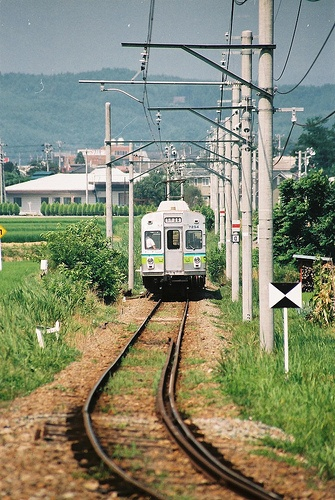
\includegraphics[width=0.7\linewidth]{fig/unnormalize/000002}
		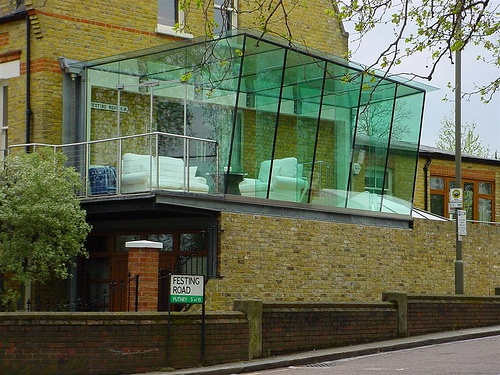
\includegraphics[width=0.8\linewidth]{fig/unnormalize/000003}
		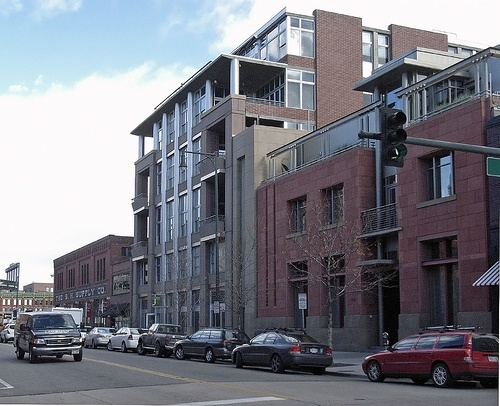
\includegraphics[width=0.8\linewidth]{fig/unnormalize/000004}
		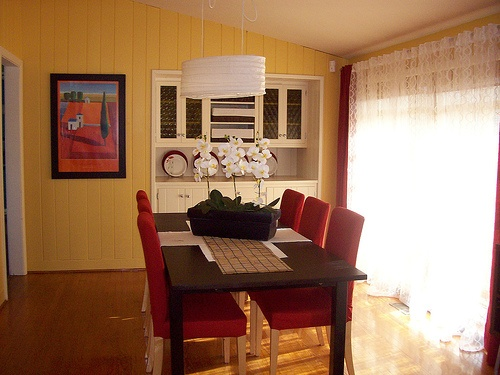
\includegraphics[width=0.8\linewidth]{fig/unnormalize/000006}
	\end{multicols}
	\begin{multicols}{4}
		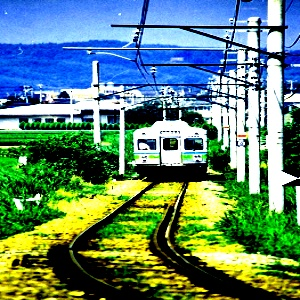
\includegraphics[width=0.8\linewidth]{fig/normalize/_1}
		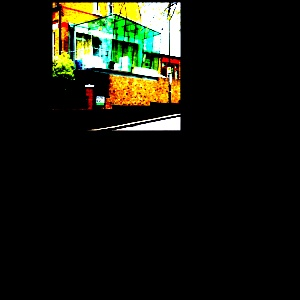
\includegraphics[width=0.8\linewidth]{fig/normalize/_2}
		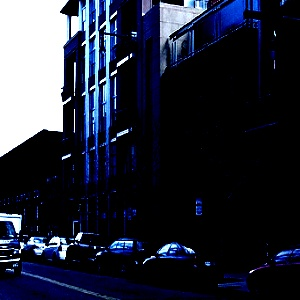
\includegraphics[width=0.8\linewidth]{fig/normalize/_3}
		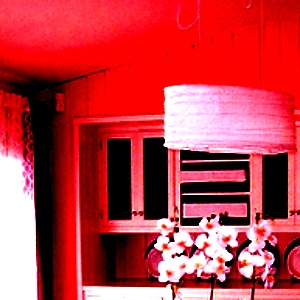
\includegraphics[width=0.8\linewidth]{fig/normalize/_4}
	\end{multicols}
	\caption{Một số hình ảnh từ tập VOC}
	\label{exampleonVOC}
\end{figure}

\subsection{\textbf{Kết quả thực nghiệm}}

Để đánh giá hiệu suất của mô hình, chúng tôi đã tiến hành các thử nghiệm trên hai tập dữ liệu quan trọng: VOC và SOHAS.

VOC là một tập dữ liệu phổ biến trong lĩnh vực nhận dạng đối tượng, bao gồm 20 lớp đối tượng khác nhau như người, xe hơi, chó, mèo, vv. Thử nghiệm trên tập dữ liệu này là một bước kiểm tra quan trọng để đánh giá khả năng khái quát hoá của mô hình. 

SOHAS là một tập dữ liệu đặc biệt, tập trung vào việc phát hiện vũ khí sát thương trong các ngữ cảnh phức tạp. Tập dữ liệu này bao gồm các hình ảnh chứa vũ khí trong các tình huống thực tế, bao gồm các vật thể che giấu, ánh sáng yếu, góc nhìn khác nhau và môi trường đa dạng. Chúng tôi sử dụng tập dữ liệu SOHAS để đánh giá khả năng của mô hình trong việc phát hiện vũ khí sát thương trong các tình huống thực tế và phức tạp.

Việc đánh giá trên cả VOC và SOHAS giúp chúng tôi có cái nhìn toàn diện về hiệu suất của mô hình. Đánh giá trên VOC đảm bảo rằng mô hình có khả năng nhận dạng và khái quát hoá tốt trên các đối tượng tổng quát. Đồng thời, đánh giá trên SOHAS đảm bảo rằng mô hình có khả năng phục vụ và giải quyết thành công bài toán phát hiện vũ khí sát thương trong các tình huống thực tế và phức tạp. 

\subsubsection{\textbf{Trên bộ dữ liệu VOC}}

Bộ dữ liệu huấn luyện được sử dụng bao gồm VOC2007 trainval (5.011 ảnh) và VOC2012 trainval (11.540 ảnh), tổng cộng 16.551 ảnh. Bộ dữ liệu kiểm thử là VOC2007 test (4.952 ảnh). Chúng tôi huấn luyện các kiến trúc mô hình của chúng tôi trong 120.000 vòng lặp (tương đương khoảng 230 epoch). Tốc độ học ban đầu là $10^{-3}$ giảm dần tại các vòng lặp 80.000 và 100.000, với hệ số $10^{-1}$. Batch size, weight decay và momentum lần lượt là 32, $5*10^-4$ và 0.9.
\begin{table*}[h]
	\caption{Mean Average Precision trên tập VOC của 4 mô hình}
	\label{mapVOC}
	\tiny
	\begin{tabularx}{\textwidth}{@{} l *{30}{C} c @{}}
		\toprule
		Model & mAP 0:5 & aero & bike & bird & boat & bottle & bus & car & cat & chair & cow & table & dog & horse & mbike & pson & plant & sheep & sofa & train & tv\\ 
		\midrule
		SSD & 77.20 & 81.10 & 84.81 & 77.57 & 70.63 & 45.81 & 85.32 & 85.69 & 89.05 & 58.60 & 81.52 & 76.92 & 86.80 & 87.50 & 84.70 & 78.51 & 51.90 & 77.15 & 78.51 & 85.84 & 76.00\\
		EMB & 78.4 & 83.6 & 85.5 & 75.9 & 71.9 & 54.2 & 87.4 & 86.8 & 87.2 & 62.8 & 82.8 & 78.8 & 85.4 & 86.4 & 85.8 & 80.2 & 51.5 & 76.9 & 81.9 & 85.7 & 77.3\\
		LFPN a & 78.27 & 83.18 & 86.12 & 78.22 & 72.05 & 51.26 & 86.95 & 86.46 & 87.76 & 59.52 & 86.05 & 75.42 & 87.72 & 87.39 & 84.66 & 79.41 & 54.22 & 78.17 & 80.24 & 85.03 & 75.60\\
		LFPN b & 78.36 & 81.97 & 84.01 & 77.10 & 71.76 & 52.37 & 86.57 & 87.02 & 88.37 & 59.71 & 87.35 & 75.35 & 88.08 & 88.49 & 85.24 & 78.94 & 52.49 & 80.23 & 78.57 & 85.19 & 78.30\\
		LFPN c & 77.69 & 82.01 & 84.35 & 78.71 & 73.39 & 51.95 & 85.58 & 86.56 & 87.41 & 57.99 & 86.28 & 73.90 & 85.40 & 87.85 & 83.98 & 78.51 & 50.95 & 78.25 & 76.66 & 85.70 & 78.34\\
		\bottomrule
		
	\end{tabularx}
\end{table*}

Bảng \ref{mapVOC} so sánh hiệu suất của Lite FPN-SSD module b (với 27.6 triệu tham số) với các mô hình khác trên tập dữ liệu VOC. Kết quả cho thấy Lite FPN-SSD module b đạt được 78.36\% mAP, vượt qua mô hình SSD gốc (77.2\% mAP với 26.3 triệu tham số) với sự cải thiện lên đến 1.16\% mAP. Mặc dù Lite FPN-SSD module b kém hơn EMB-SSD \cite{ssdemb} 0.04\% mAP, nhưng nó có số lượng tham số ít hơn đáng kể (2 triệu tham số). Điều này cho thấy Lite FPN-SSD module b là một lựa chọn hiệu quả và tiết kiệm tài nguyên cho việc nhận dạng đối tượng trên tập dữ liệu VOC. Rõ ràng rằng Lite FPN-SSD module b đạt được một hiệu suất tốt và cân bằng giữa số lượng tham số, giúp mô hình trở nên nhẹ nhàng và dễ dàng triển khai trên các thiết bị có tài nguyên hạn chế.

\begin{figure}[h]
	\centering
	\includegraphics[width=0.7\linewidth]{fig/VOC_mAP}
	\caption{Hiệu suất giữa ba mô hình trên tập dữ liệu VOC}
	\label{fig:vocmap}
\end{figure}


\begin{figure}[h]
	\center
	\begin{multicols}{2}
		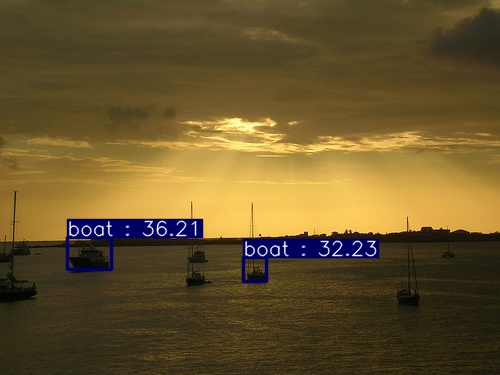
\includegraphics[width=0.7\linewidth]{fig/VOC_41}
		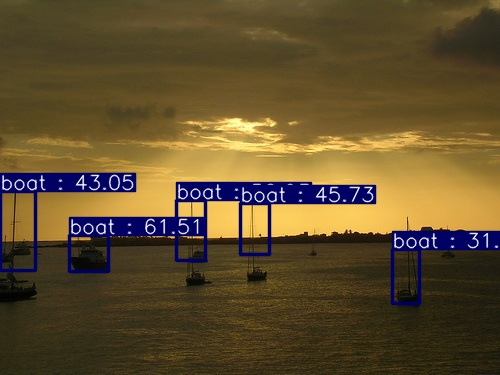
\includegraphics[width=0.7\linewidth]{fig/VOC_FPN_41}
	\end{multicols}
	\begin{multicols}{2}
		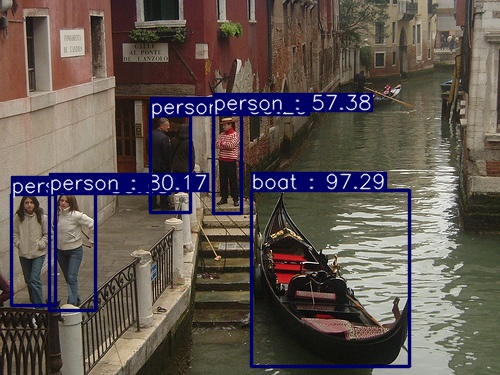
\includegraphics[width=0.7\linewidth]{fig/VOC_578}
		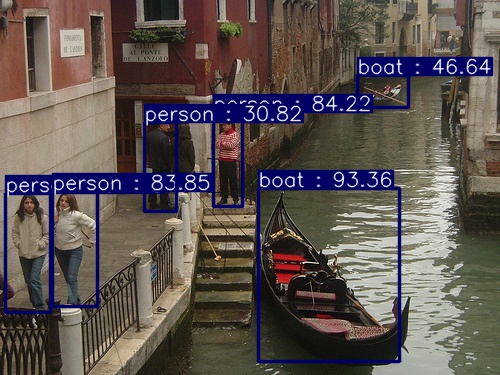
\includegraphics[width=0.7\linewidth]{fig/VOC_FPN_578}
	\end{multicols}
	\begin{multicols}{2}
		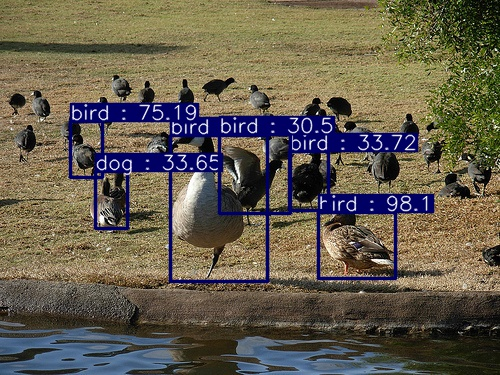
\includegraphics[width=0.7\linewidth]{fig/VOC_638}
		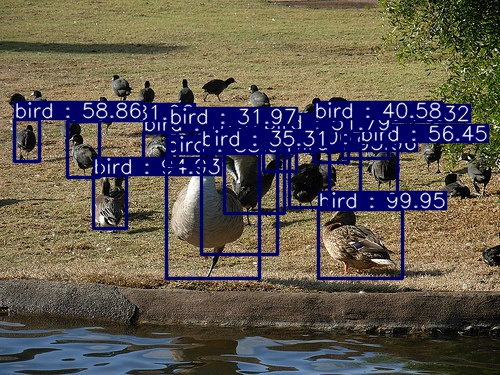
\includegraphics[width=0.7\linewidth]{fig/VOC_FPN_638}
	\end{multicols}
	\begin{multicols}{2}
		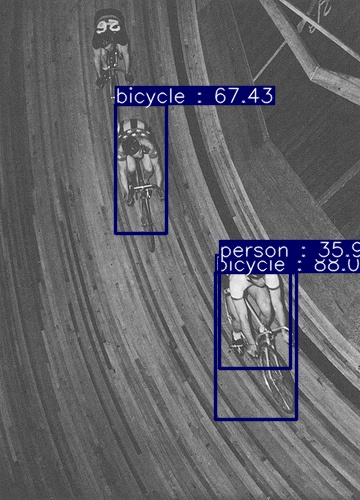
\includegraphics[width=0.7\linewidth]{fig/VOC_78}
		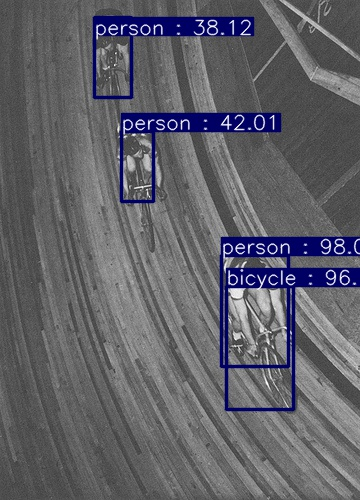
\includegraphics[width=0.7\linewidth]{fig/VOC_FPN_78}
	\end{multicols}
	\captionsetup{justification=centering}
	\caption{Kết quả trên tập VOC của SSD gốc (trái) và Lite FPN SSD (phải)}
	\label{onVOC}
\end{figure} 

\subsubsection{\textbf{Trên bộ dữ liệu SOHAS}}

Tập huấn luyện bao gồm khoảng 5.000 ảnh, tập kiểm tra bao gồm khoảng 800 ảnh. Nó được thiết kế đặc biệt để phát hiện vũ khí trong các tình huống thực tế. Nhằm đáp đáp ứng mục tiêu của nghiên cứu, khác với bài báo đã được công bố, chúng tôi tiến thành huấn luyện lại mô hình với 45.000 vòng lặp, tốc độ học ban đầu là $10^{-4}$, giảm dần ở vòng lặp 20.000 và 35.000 với hệ số $10^{-1}$. 

Chịu sự ảnh hưởng từ các điều kiện môi trường (ánh sáng, góc quay, độ phân giải ... xem hình \ref{onSOHAS}) trong thực tế từ tập dữ liệu SOHAS, Lite FPN-SSD vẫn đạt được mAP rất lên đến 71.93\% (bảng \ref{mAPSOHAS}).. Với kết quả này, Lite FPN-SSD có thể được triển khai hiệu quả để cải thiện an ninh và đảm bảo an toàn trong các môi trường đòi hỏi sự phát hiện và ngăn chặn vũ khí.

\begin{table*}[h]
	\caption{Mean Average Precision trên SOHAS}
	\label{mAPSOHAS}
	\begin{tabularx}{\textwidth}{@{} l *{10}{C} c @{}}
		\toprule
		Model & mAP & Pistol & Phone & Knife & Purse & Money & Card \\
		\midrule
		Lite FPN SSD & 71.93 & 77.34 & 72.47 & 86.86 & 71.14 & 76.40 & 47.36 \\ 
		\bottomrule
	\end{tabularx}
\end{table*}

\begin{figure}[h]
	\center
	\begin{multicols}{2}
		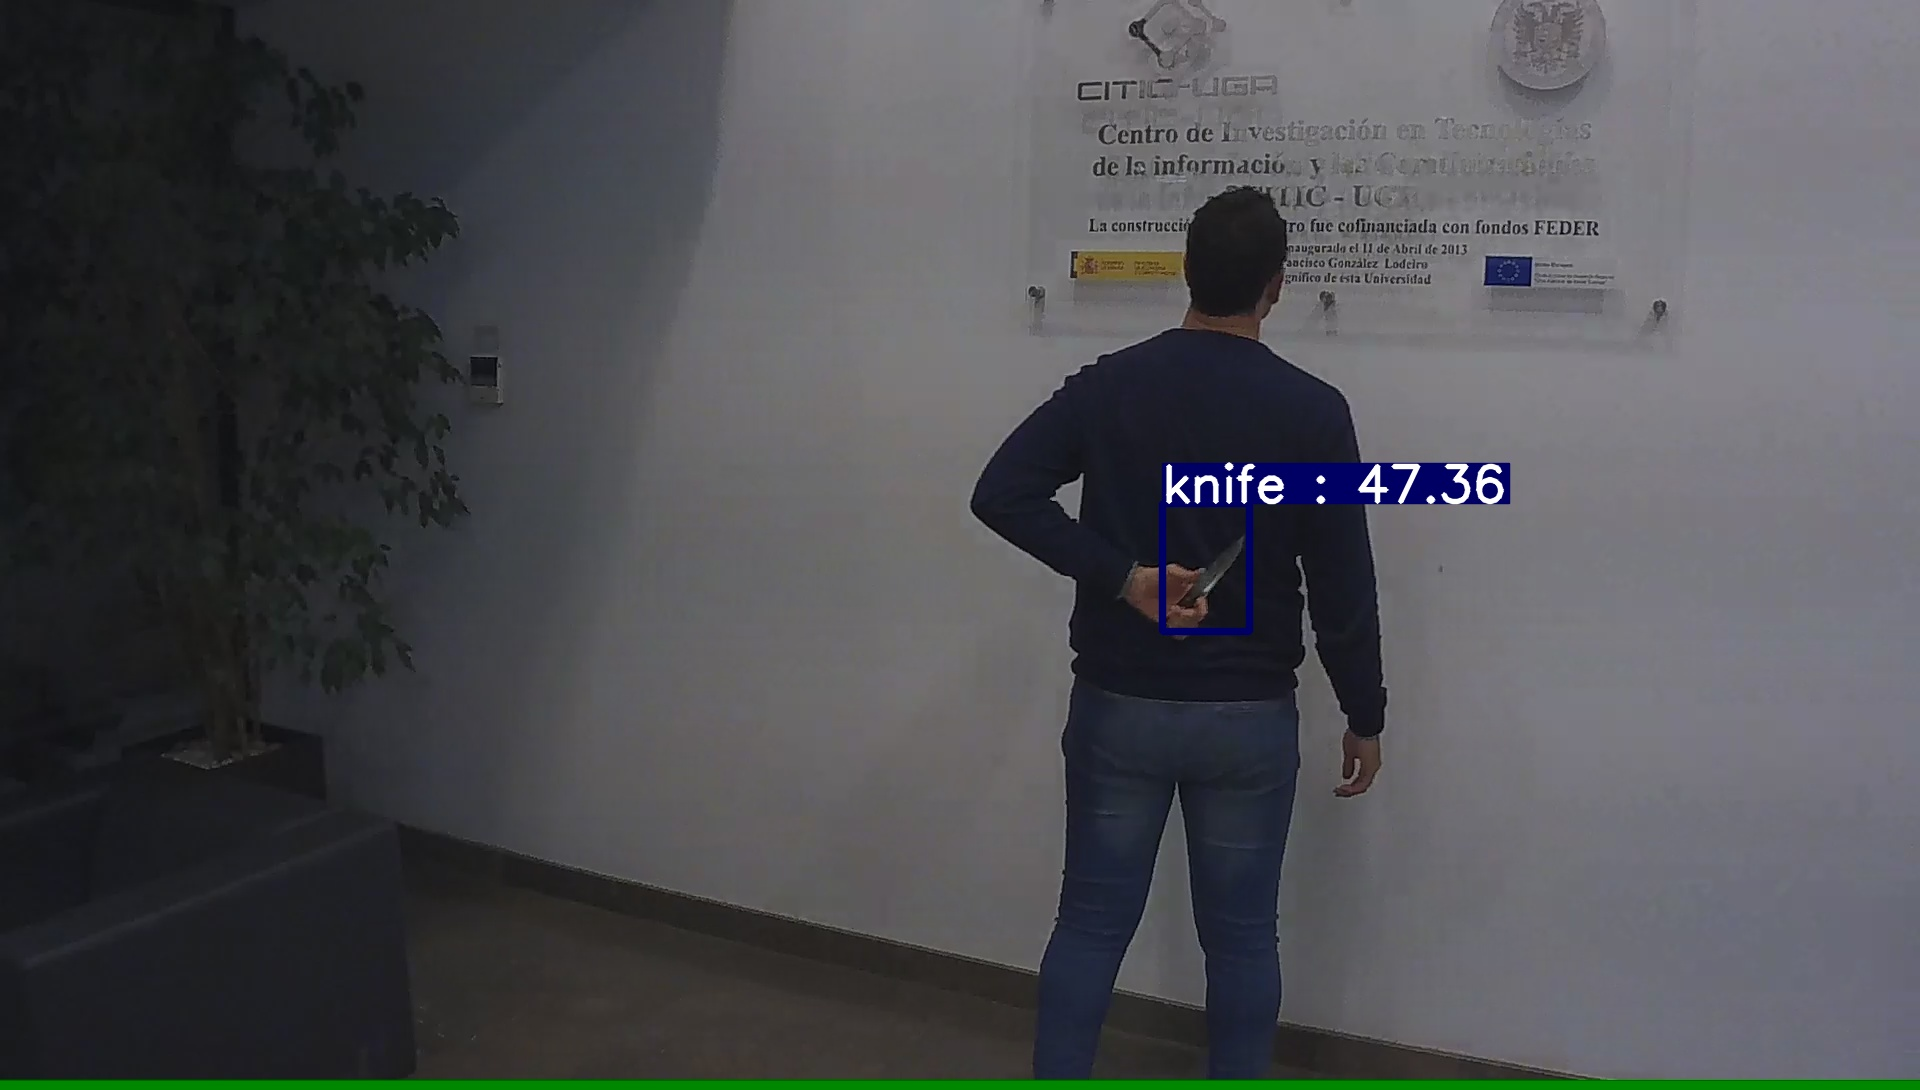
\includegraphics[width=1.\linewidth]{fig/SOHAS_9}
		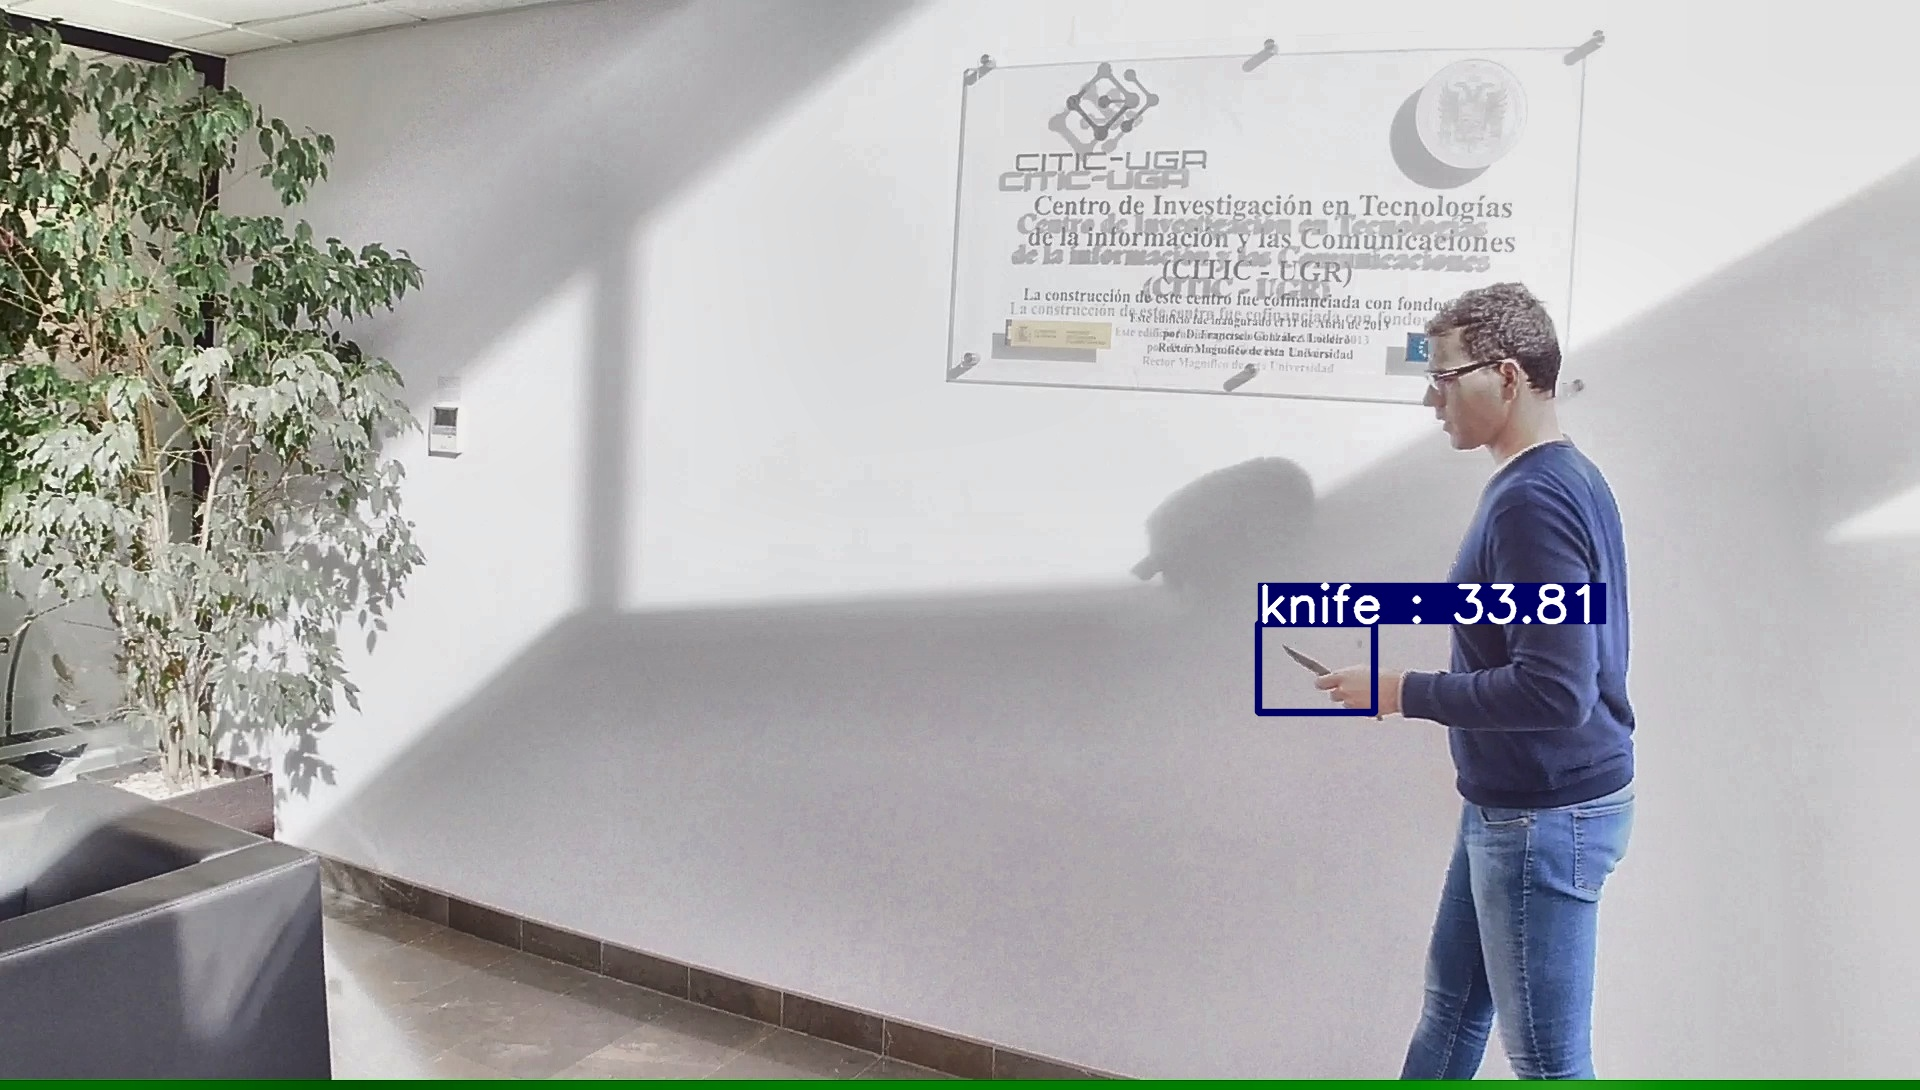
\includegraphics[width=1.\linewidth]{fig/SOHAS_104}
	\end{multicols}
	\begin{multicols}{2}
		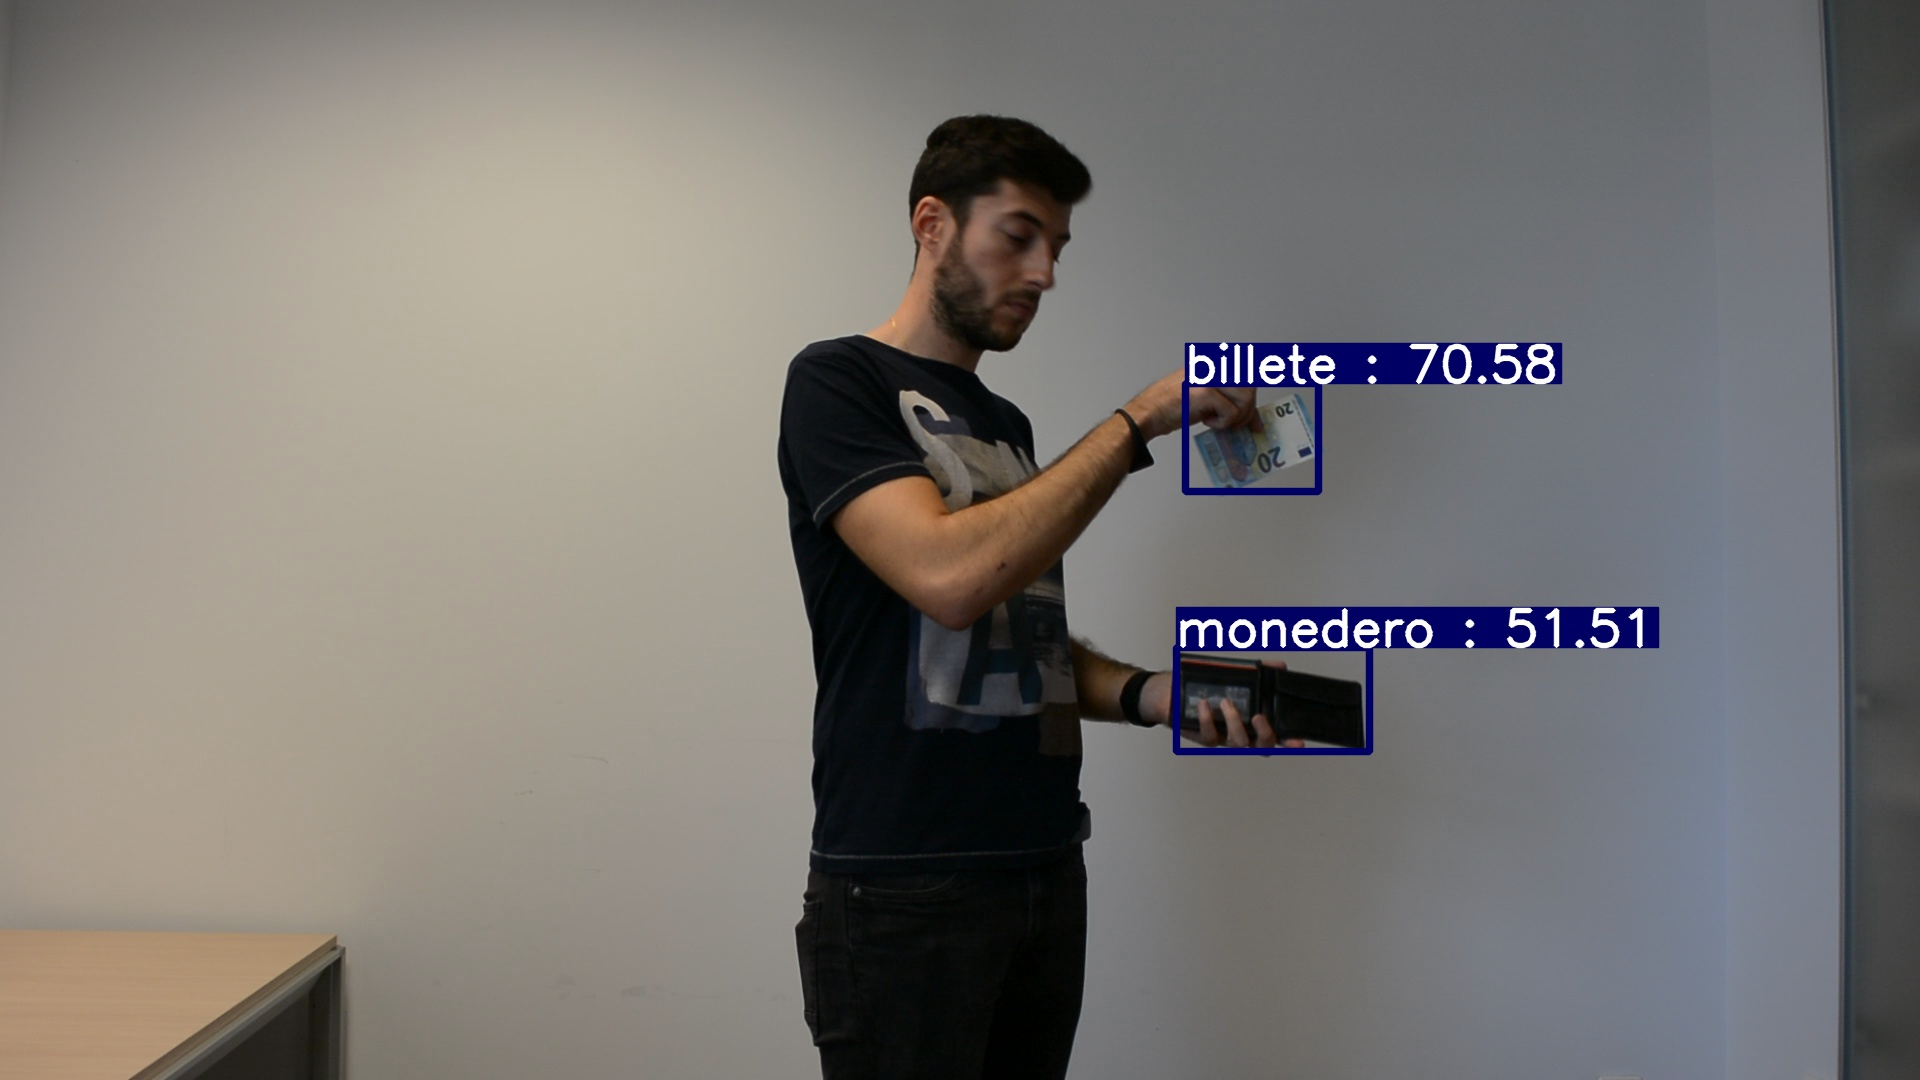
\includegraphics[width=1.\linewidth]{fig/SOHAS_133}
		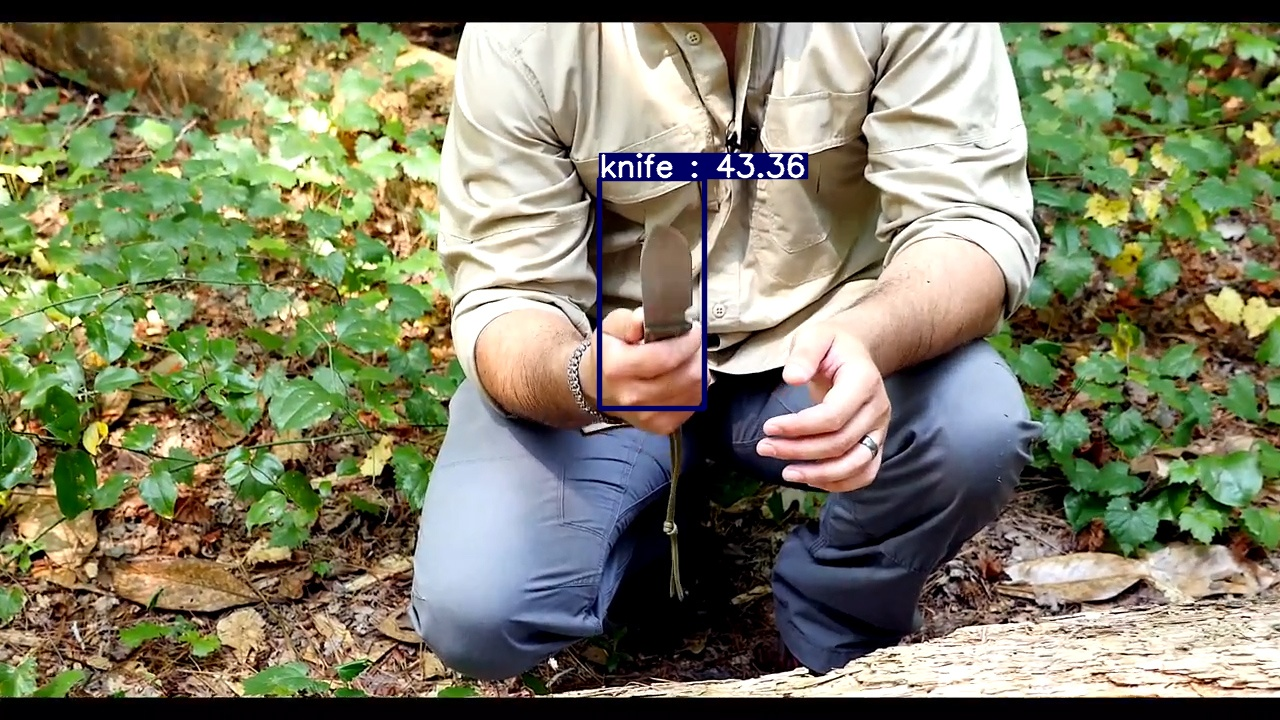
\includegraphics[width=1.\linewidth]{fig/SOHAS_257}
	\end{multicols}
	\begin{multicols}{2}
		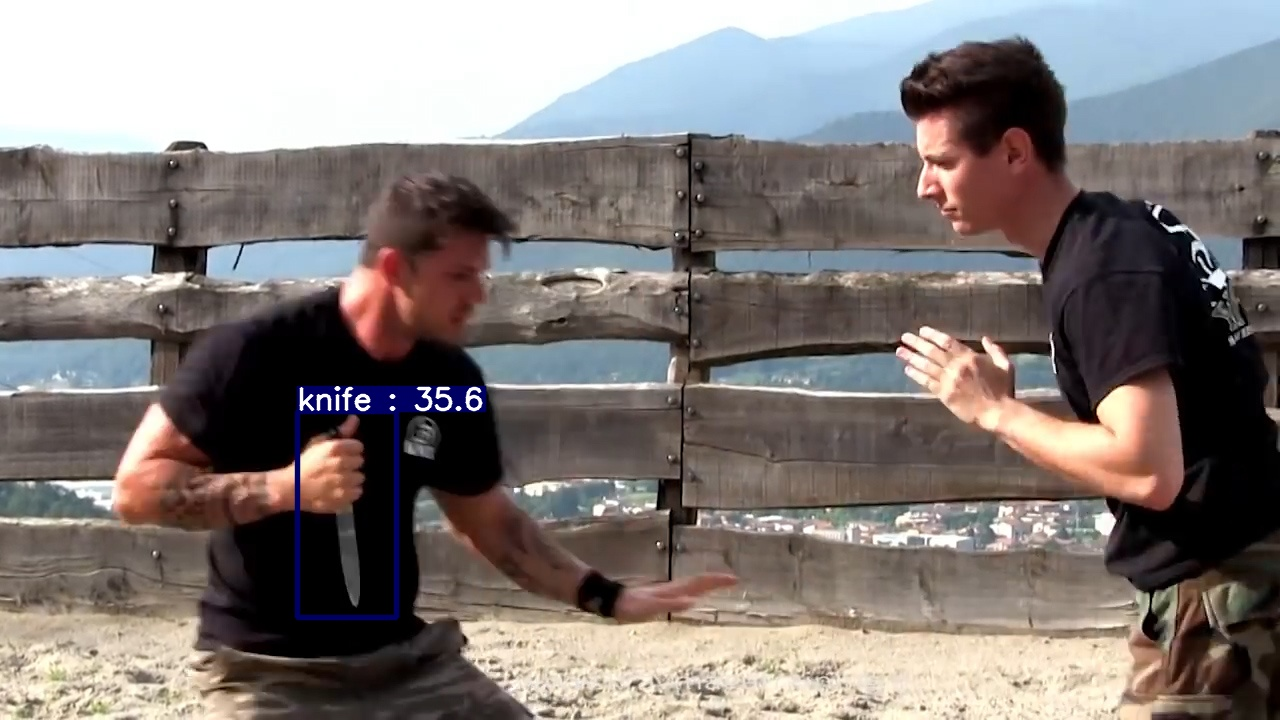
\includegraphics[width=1.\linewidth]{fig/SOHAS_561}
		\includegraphics[width=1.\linewidth]{fig/SOHAS_653}
	\end{multicols}
	\begin{multicols}{2}
		\includegraphics[width=1.\linewidth]{fig/SOHAS_1}
		\includegraphics[width=1.\linewidth]{fig/SOHAS_711}
	\end{multicols}
	\caption{Kết quả trên tập SOHAS của Lite FPN SSD}
	\label{onSOHAS}
\end{figure}

\section{\textbf{Kết luận và hướng phát triển}}

Chúng tôi đã đề xuất và chứng minh tính hiệu quả của mô hình Lite FPN-SSD. Bằng cách tổng hợp thông tin từ các lớp đặc trưng nông và sâu thông qua kết hợp mô hình SSD và kiến trúc mạng phân tầng kim tự tháp cùng với mô-đun FPN, lớp đặc trưng mới mang nhiều thông tin ngữ nghĩa hơn. Qua thực nghiệm trên tập dữ liệu VOC, chúng tôi đã chứng minh được mô hình đề xuất có hiệu suất phát hiện và nhận diện đối tượng tốt hơn. Lite FPN-SSD cải thiện mức mAP đáng kể (78.36\% so với 77.2\%) trong khi không tác động đáng kể để tốc độ khi chỉ yêu cầu thêm 2 triệu tham số. Sau khi được đánh giá trên tập dữ liệu tổng quát, chúng tôi áp dụng mô hình đề xuất lên tập dữ liệu nhận diện vũ khí với ngữ cảnh phức tạp : SOHAS. Kết quả cho thấy Lite FPN-SSD hoàn toàn đạt được khả năng khái quát hóa và phù hợp cho các tác vụ mang tính cụ thể như nhận diện vũ khí sát thương trong thời gian thực, đáp ứng được mục ban đầu của nghiên cứu.

Với khả năng tùy biến và thiết kế linh hoạt của Feature Pyramid Network (FPN) và module FPN, Lite FPN-SSD mở ra nhiều cơ hội mở rộng và tinh chỉnh mô hình theo nhu cầu và mục đích sử dụng cụ thể. Cụ thể, nếu muốn mục tiêu là tối ưu độ chính xác, có thể lựa chọn lối thiết kế FPN phức tạp hơn (sử dụng skip connection, cross connection ...) hay chọn một FPN module mạnh mẽ hơn. Nếu mục tiêu là tối ưu tốc độ, có thể xem xét các mạng xương sống nhẹ mà vẫn hiệu quả như MobileNet \cite{mobilenets}. Điều này tạo ra một nền tảng vững chắc cho các nghiên cứu tiếp theo, đồng thời khuyến khích thử nghiệm và cải tiến để đạt được hiệu suất tốt hơn.

\addcontentsline{toc}{section}{6\quad Tài liệu tham khảo}
\renewcommand\refname{Tài liệu tham khảo}

\bibliographystyle{ieeetr}
\bibliography{references.bib}

\end{document}
